% Options for packages loaded elsewhere
\PassOptionsToPackage{unicode}{hyperref}
\PassOptionsToPackage{hyphens}{url}
\PassOptionsToPackage{dvipsnames,svgnames,x11names}{xcolor}
\documentclass[
  11pt,
]{article}
\usepackage{xcolor}
\usepackage[margin=1in]{geometry}
\usepackage{amsmath,amssymb}
\setcounter{secnumdepth}{-\maxdimen} % remove section numbering
\usepackage{iftex}
\ifPDFTeX
  \usepackage[T1]{fontenc}
  \usepackage[utf8]{inputenc}
  \usepackage{textcomp} % provide euro and other symbols
\else % if luatex or xetex
  \usepackage{unicode-math} % this also loads fontspec
  \defaultfontfeatures{Scale=MatchLowercase}
  \defaultfontfeatures[\rmfamily]{Ligatures=TeX,Scale=1}
\fi
\usepackage{lmodern}
\ifPDFTeX\else
  % xetex/luatex font selection
\fi
% Use upquote if available, for straight quotes in verbatim environments
\IfFileExists{upquote.sty}{\usepackage{upquote}}{}
\IfFileExists{microtype.sty}{% use microtype if available
  \usepackage[]{microtype}
  \UseMicrotypeSet[protrusion]{basicmath} % disable protrusion for tt fonts
}{}
\makeatletter
\@ifundefined{KOMAClassName}{% if non-KOMA class
  \IfFileExists{parskip.sty}{%
    \usepackage{parskip}
  }{% else
    \setlength{\parindent}{0pt}
    \setlength{\parskip}{6pt plus 2pt minus 1pt}}
}{% if KOMA class
  \KOMAoptions{parskip=half}}
\makeatother
\usepackage{longtable,booktabs,array}
\newcounter{none} % for unnumbered tables
\usepackage{calc} % for calculating minipage widths
% Correct order of tables after \paragraph or \subparagraph
\usepackage{etoolbox}
\makeatletter
\patchcmd\longtable{\par}{\if@noskipsec\mbox{}\fi\par}{}{}
\makeatother
% Allow footnotes in longtable head/foot
\IfFileExists{footnotehyper.sty}{\usepackage{footnotehyper}}{\usepackage{footnote}}
\makesavenoteenv{longtable}
\usepackage{graphicx}
\makeatletter
\newsavebox\pandoc@box
\newcommand*\pandocbounded[1]{% scales image to fit in text height/width
  \sbox\pandoc@box{#1}%
  \Gscale@div\@tempa{\textheight}{\dimexpr\ht\pandoc@box+\dp\pandoc@box\relax}%
  \Gscale@div\@tempb{\linewidth}{\wd\pandoc@box}%
  \ifdim\@tempb\p@<\@tempa\p@\let\@tempa\@tempb\fi% select the smaller of both
  \ifdim\@tempa\p@<\p@\scalebox{\@tempa}{\usebox\pandoc@box}%
  \else\usebox{\pandoc@box}%
  \fi%
}
% Set default figure placement to htbp
\def\fps@figure{htbp}
\makeatother
% definitions for citeproc citations
\NewDocumentCommand\citeproctext{}{}
\NewDocumentCommand\citeproc{mm}{%
  \begingroup\def\citeproctext{#2}\cite{#1}\endgroup}
\makeatletter
 % allow citations to break across lines
 \let\@cite@ofmt\@firstofone
 % avoid brackets around text for \cite:
 \def\@biblabel#1{}
 \def\@cite#1#2{{#1\if@tempswa , #2\fi}}
\makeatother
\newlength{\cslhangindent}
\setlength{\cslhangindent}{1.5em}
\newlength{\csllabelwidth}
\setlength{\csllabelwidth}{3em}
\newenvironment{CSLReferences}[2] % #1 hanging-indent, #2 entry-spacing
 {\begin{list}{}{%
  \setlength{\itemindent}{0pt}
  \setlength{\leftmargin}{0pt}
  \setlength{\parsep}{0pt}
  % turn on hanging indent if param 1 is 1
  \ifodd #1
   \setlength{\leftmargin}{\cslhangindent}
   \setlength{\itemindent}{-1\cslhangindent}
  \fi
  % set entry spacing
  \setlength{\itemsep}{#2\baselineskip}}}
 {\end{list}}
\usepackage{calc}
\newcommand{\CSLBlock}[1]{\hfill\break\parbox[t]{\linewidth}{\strut\ignorespaces#1\strut}}
\newcommand{\CSLLeftMargin}[1]{\parbox[t]{\csllabelwidth}{\strut#1\strut}}
\newcommand{\CSLRightInline}[1]{\parbox[t]{\linewidth - \csllabelwidth}{\strut#1\strut}}
\newcommand{\CSLIndent}[1]{\hspace{\cslhangindent}#1}
\setlength{\emergencystretch}{3em} % prevent overfull lines
\providecommand{\tightlist}{%
  \setlength{\itemsep}{0pt}\setlength{\parskip}{0pt}}
\usepackage{setspace}
\setstretch{1.5}
\usepackage{indentfirst}
\setlength{\parindent}{10pt}
\usepackage{authblk}
\usepackage{booktabs}
\usepackage{caption}
\usepackage{dcolumn}
\usepackage{adjustbox}
\usepackage{threeparttable}
\usepackage{pdflscape}
\usepackage{float}
\usepackage{fancyhdr}
\pagestyle{fancy}
\fancyhf{}
\setlength{\headheight}{14pt}
\addtolength{\topmargin}{-2pt}
\fancyhead[L]{\small\scshape Asymmetric Climate Impacts on Fishing Effort}
\fancyhead[R]{\small\thepage}
\renewcommand{\headrulewidth}{0.4pt}
\usepackage{etoolbox}
\AtBeginEnvironment{CSLReferences}{\small\setstretch{1.0}}
\BeforeBeginEnvironment{abstract}{\begin{spacing}{1.5}}
\AfterEndEnvironment{abstract}{\end{spacing}}
\author{Felipe J. Quezada-Escalona\thanks{Associate Professor, Department of Economics, Universidad de Concepci\'on. Mailing address: Victoria 471, Concepci\'on, Chile. Email: felipequezada@udec.cl; Adjunct Researcher, Interdisciplinary Center for Aquaculture Research---Applied Research (INCAR\textsuperscript{2}), Universidad de Concepci\'on, Chile.}}
\affil{Universidad de Concepci\'on \vspace{-60pt}}
\newcommand{\keywords}[1]{\par\noindent{\setstretch{1.5}\textbf{Keywords:} #1\par}}
\newcommand{\jelcodes}[1]{\par\noindent{\setstretch{1.5}\textbf{JEL Codes:} #1\par}}
\usepackage{bookmark}
\IfFileExists{xurl.sty}{\usepackage{xurl}}{} % add URL line breaks if available
\urlstyle{same}
\hypersetup{
  pdftitle={Differential Climate Impacts on Fishing Effort in Chilean Small Pelagic Fisheries},
  pdfauthor={Felipe J. Quezada-Escalona},
  colorlinks=true,
  linkcolor={blue},
  filecolor={Maroon},
  citecolor={blue},
  urlcolor={blue},
  pdfcreator={LaTeX via pandoc}}

\title{Differential Climate Impacts on Fishing Effort in Chilean Small Pelagic Fisheries}
\author{Felipe J. Quezada-Escalona}
\date{June 2026}

\begin{document}
\maketitle
\begin{abstract}
Climate-driven shifts in stock productivity reach fishing fleets unevenly when species portfolios differ across segments and vessel range determines which stocks each fleet can access. We measure this asymmetry for Chile's Central-South small pelagic fishery (anchoveta, sardine, jack mackerel), under a fixed industrial-artisanal allocation with active cessions. A Bayesian state-space stock-dynamics model fit to 2000-2024 assessments is coupled with a vessel-level trip equation; climate enters via an indirect biomass channel and a direct weather channel. Under a six-model CMIP6 ensemble, projected effort falls by 16-18 percent for the artisanal fleet but only 0.8-1.0 percent for the industrial fleet---an asymmetry of seventeen to one, driven by the artisanal fleet's exposure to the two coastal stocks whose climate shifters are large and identified. Climate-adaptation policy should target the artisanal segment: its restricted range prevents access to offshore jack mackerel when coastal stocks collapse, while the industrial fleet retains that access.
\end{abstract}

\par\noindent{\setstretch{1.5}\textbf{Keywords:} Bayesian state-space model; Bioeconomic projection; Chilean small pelagic fishery; Climate change; Fishing effort; Fleet heterogeneity; Quota allocation\par}

\par\noindent{\setstretch{1.5}\textbf{JEL Codes:} Q22, Q54, Q57, Q58\par}

\doublespacing

\section{Introduction}\label{introduction}

Climate change is reshaping the productivity of marine fisheries, but the burden falls unevenly across fleet segments. When species portfolios differ across segments and vessel range determines which stocks each fleet can access, the climate-induced loss concentrates in the segment whose accessible stocks are most exposed. The empirical literature has rarely delivered fleet-level effort projections that respect this technological constraint, particularly for multi-species fisheries managed under sector-asymmetric allocation regimes.

We provide such projections for the small pelagic fishery (SPF) of Central-South Chile (from Valparaíso to Los Lagos), part of the country's largest fishery---approximately \(86\%\) of national landings in 2019 (\citeproc{ref-SUBPESCA2020}{SUBPESCA 2020})---and the only zone where all three target species, anchoveta (\emph{Engraulis ringens}), sardine (\emph{Strangomera bentincki}; locally sardina común), and jack mackerel (\emph{Trachurus murphyi}; locally jurel), coexist in non-negligible shares of both fleet portfolios (\citeproc{ref-Alheit2004}{Alheit and Niquen 2004}; \citeproc{ref-Arancibia2019-FIPA}{Arancibia et al. 2019}; \citeproc{ref-dresdner2013}{Dresdner et al. 2013}). The fishery is managed through a fixed industrial--artisanal allocation of the Total Allowable Catch, with administratively rationed but heavily used inter-sectoral cessions: industrial titulares cede most of their anchoveta and sardine quota to artisanal cessionaries each year (Online Appendix F). Within-sector distribution operates through Transferable Fishing Licenses (\emph{Licencias Transables de Pesca}, LTP) for the industrial fleet and the Artisanal Extraction Regime (\emph{Régimen Artesanal de Extracción}, RAE) for the artisanal fleet. The two fleets target distinct portfolios shaped by vessel size and range: industrial purse-seiners operate offshore primarily on jack mackerel, while the smaller-vessel artisanal fleet operates in coastal waters primarily on anchoveta and sardine. Under climate stress, this technological--geographical specialisation determines which stocks each fleet can access. Cross-country evidence projects moderate declines in Chile's maximum catch potential (6--13\% by 2055; Cheung et al. (\citeproc{ref-Cheung2010}{2010})), and the climate-fisheries economics literature is concentrated in a few well-studied regions (\citeproc{ref-sumaila2011}{Sumaila et al. 2011}). To our knowledge, no existing study for Chile combines multi-species stock dynamics with vessel-level effort responses under projected climate scenarios.\footnote{The only empirical study of Chilean fisher behavior that we are aware of is Peña-Torres et al. (\citeproc{ref-Pena-Torres2017-gn}{2017}), which analyses how the El Niño--Southern Oscillation (ENSO) affects location choices in the jack mackerel fishery.}

Our bioeconomic framework combines two empirical components. First, a Bayesian state-space model of multi-species stock dynamics, fitted to 2000--2024 official assessments from the Chilean Fisheries Development Institute (IFOP) and the South Pacific Regional Fisheries Management Organisation (SPRFMO), estimates for each species two semi-elasticities of productivity with respect to sea-surface temperature and log-chlorophyll-a anomalies---parameters we call \emph{climate shifters}. Because they enter the biological law of motion as coefficients on exogenous climate forcings, they retain a structural interpretation when applied to climate states outside the 2000--2024 sample. Second, a vessel-level negative binomial trip equation, estimated separately for the industrial and artisanal fleets with year fixed effects, maps prices, allocated harvest, weather, and regulatory closures into annual fishing effort. Climate reaches fleet-level effort through two channels: an \emph{indirect biomass channel} via the climate shifters and a \emph{direct weather channel} via vessel-specific exposure to severe winds. We evaluate the framework against a six-model CMIP6 ensemble under SSP2-4.5 and SSP5-8.5 at mid-century (2041--2060) and end-of-century (2081--2100).

We obtain three sets of results. First, the artisanal segment absorbs most of the projected climate impact: fleet-level effort falls by \(16\)--\(18\%\) for artisanal vessels but only \(0.8\)--\(1.0\%\) for industrial vessels under SSP5-8.5, an asymmetry of roughly seventeen to one. Second, the asymmetry is driven by differential portfolio exposure combined with the artisanal fleet's restricted operating range: artisanal vessels concentrate in anchoveta and sardine (whose climate shifters are large and well-identified) and lack offshore access to jack mackerel, while \(95\%\) of industrial activity sits in jack mackerel whose Centro-Sur climate shifter the data cannot identify. Third, the within-artisanal heterogeneity is itself substantial: the dominant \emph{lancha motor} segment contracts by \(-19.6\%\) under SSP5-8.5 end-of-century while the smaller \emph{bote motor} segment contracts by \(-10.0\%\), reflecting differential absolute exposure to the collapsing coastal stocks rather than differences in elasticity.

The remainder of the paper is organized as follows. The next section describes the economic and institutional setting of the Chilean SPF. We then present the empirical framework --- data, stock-dynamics model, trip equation, and projection design --- followed by results on identified climate shifters, comparative-statics projections of stock productivity, and projections of fleet-level effort. The paper closes with a discussion of policy implications and limitations, and brief concluding remarks.

\section{The small pelagic fishery in Chile}\label{the-small-pelagic-fishery-in-chile}

The fishery is divided into two latitudinal zones with distinct species compositions. The northern zone (from Arica y Parinacota to Coquimbo) is dominated by anchoveta and jack mackerel, while sardine is effectively absent. In contrast, the Central-South zone (from Valparaíso to Los Lagos) includes all three species in non-negligible shares within both artisanal and industrial landings. Because this region supports a genuinely multi-species fishery operating under a fixed sector-level allocation regime, it provides the relevant setting for evaluating the distributional consequences of climate-induced shifts in stock productivity, and is therefore the focus of this paper. The principal ports servicing this zone include San Antonio, Tomé, Talcahuano, San Vicente, Coronel, Lota, and Corral. The three species are harvested primarily by purse-seine fleets that differ in vessel size, operating range, and species composition. Median catch composition differs sharply across fleets: artisanal vessels are concentrated in sardine (\(\sim 81\%\) of catch) and anchoveta (\(\sim 18\%\)), with negligible jack mackerel; the industrial fleet is the inverse, with \(\sim 95\%\) jack mackerel and \(\sim 5\%\) sardine.

The historical evolution of the fishery illustrates the portfolio mechanism developed in the remainder of the paper. The jack mackerel fishery was initially concentrated in northern Chile but shifted toward the Central-South zone during the mid-1980s (\citeproc{ref-Pena-Torres2017-gn}{Peña-Torres et al. 2017}), where fishing grounds have traditionally operated within 50 nautical miles of the coast. Between 1987 and 2004, approximately 85\% of jack mackerel landings were directed to the reduction industry (\citeproc{ref-Pena-Torres2017-gn}{Peña-Torres et al. 2017}), reflecting the importance of fishmeal and fish-oil export markets in determining the value of the industrial portfolio. Sardine and anchoveta, by contrast, are jointly harvested using the same gear and fishing grounds. The two species share habitat and fishing technology, making species differentiation at the point of capture effectively impossible (\citeproc{ref-dresdner2013}{Dresdner et al. 2013}). As a result, the binding constraint on the species mix of landings is the quota regime, not biology or technology.

The status of the three stocks has evolved substantially over time. Central-South anchoveta was classified as collapsed through 2018, reclassified as overexploited in 2019, and has been harvested within maximum sustainable yield (MSY) limits since 2020. Sardine has generally remained within MSY reference levels, except in 2021 and 2023 when it was classified as overexploited. Jack mackerel remained overexploited until 2018 and has since been harvested within MSY limits.

Biological closures (\emph{vedas}) constitute a central management instrument for sardine and anchoveta. In the Central-South zone, reproductive closures extend from July to October in Araucanía--Los Lagos and from August to October in Valparaíso--Biobío, while recruitment closures occur from January through February across all regions. In total, these regulations generate 151 closed fishing days per year in Valparaíso--Biobío and 182 days in Araucanía--Los Lagos. Jack mackerel is not subject to seasonal biological closures.

The Chilean SPF is managed through an annual Total Allowable Catch (TAC; \emph{Cuota Global}), further subdivided across regions and seasons, with unused quotas reassignable within the fishing year and small fractions reserved for research and contingency. Anchoveta and sardine operate under a mixed-species quota framework in which each species has an independent quota but substitution between them is permitted.

The partition of each TAC between the industrial and artisanal sectors is fixed by statute. The pre-reform partition governed the de jure allocation during the estimation window (2013--2024); a 2025 reform (\citeproc{ref-Ley21752-2025}{Congreso Nacional de Chile 2025}) fixes a new partition in force until 2040 (Table \ref{tab:fractioning}). Under the pre-reform regime, the artisanal sector held \(78\%\) of the Central-South anchoveta and sardine TACs and \(10\%\) of the jack mackerel TAC; the 2025 reform raises the anchoveta and sardine artisanal shares to \(90\%\) across Valparaíso--Los Lagos, and the jack mackerel artisanal share to \(30\%\) in Valparaíso--Los Ríos and \(15\%\) in Los Lagos. The de jure partition admits a single administratively rationed inter-sectoral re-allocation channel, subject to ex-ante authorisation by the Subsecretaría de Pesca y Acuicultura (SUBPESCA). Quota control reports from the Servicio Nacional de Pesca y Acuicultura (SERNAPESCA) for \(2013\)--\(2024\) document that the industrial sector cedes a persistently large share of its assigned anchoveta and sardine TACs to artisanal cessionaries --- from \(12\)--\(72\%\) over \(2013\)--\(2017\), tightening to \(85\)--\(99\%\) every year in \(2018\)--\(2024\) (Online Appendix, Table F.3) --- while jack mackerel cessions are an order of magnitude smaller and shift direction across years (Online Appendix, Table F.4). Our empirical specifications are therefore identified on realised landings, which are post-cession: the post-cession allocation reflects the joint statutory--cession regime, not the de jure fractioning alone.

Within the industrial sector, an individual transferable quota (ITQ) system known as Transferable Fishing Licenses (\emph{Licencias Transables de Pesca}, LTP) has operated since 2013: Class A licenses were allocated according to historical catch shares, whereas Class B licenses---up to 15\% of the industrial allocation---have been distributed through sealed-bid first-price auctions since 2015.\footnote{Peña-Torres et al. (\citeproc{ref-peuxf1a_torres_2022_MRE}{2022}) document that these Class B auctions have exhibited low participation, limited capacity to reflect economies of scale, and indications of coordinated bidding.} The artisanal sector operates under a limited-entry regime, with regional TACs distributed through the \emph{Régimen Artesanal de Extracción} (RAE) according to area, vessel size, landing site, or fisher organization. Since 2004, the RAE admits voluntary cooperative catch shares within fisher organizations (\citeproc{ref-ChavezEstrada2018-ccs}{Chávez Estrada et al. 2018}). By statute, the first five nautical miles from the coastline constitute an exclusive artisanal reserve area, off-limits to industrial vessels (\citeproc{ref-ChavezEstrada2018-ccs}{Chávez Estrada et al. 2018}). Artisanal vessels (up to \(18\) m length) are not legally confined to that zone, but their effective operating range is constrained by vessel size and operational autonomy (fuel and storage capacity), restricting them in practice to coastal waters where anchoveta and sardine concentrate within roughly \(30\) km of the coast (\citeproc{ref-ChavezEstrada2018-ccs}{Chávez Estrada et al. 2018}). The larger industrial purse-seine fleet operates across the broader exclusive economic zone (up to \(200\) nautical miles offshore), where jack mackerel is typically found in offshore waters; under El Niño events the stock extends beyond the EEZ to more than \(1{,}000\) nautical miles off the central Chilean coast (\citeproc{ref-Pena-Torres2017-gn}{Peña-Torres et al. 2017}). This technological--geographical specialisation makes the offshore jack mackerel stock effectively inaccessible to the artisanal fleet.

\begin{table}[H]
\centering
\caption{Statutory sectoral partition of the Central-South small pelagic TACs, pre- and post-2025 reform.\label{tab:fractioning}}
\begin{threeparttable}
\begin{tabular}{lcc}
\toprule
 & \multicolumn{2}{c}{Artisanal share of TAC (\%)} \\
\cmidrule(lr){2-3}
Stock & Pre-reform & 2025 reform \\
\midrule
Anchoveta (Valparaíso--Los Lagos)             & $78$ & $90$ \\
Sardina com\'un (Valparaíso--Los Lagos)       & $78$ & $90$ \\
Jack mackerel (Valparaíso--Los Ríos)                  & $10$ & $30$ \\
Jack mackerel (Los Lagos)                             & $10$ & $15$ \\
\bottomrule
\end{tabular}
\begin{tablenotes}[para,flushleft]
\footnotesize
\item \emph{Notes.} Sources: SERNAPESCA (2024) for the pre-2025 regime and Congreso Nacional de Chile (2025) for the 2025 reform, in force until 31 December 2040.
\end{tablenotes}
\end{threeparttable}
\end{table}

\section{Methods}\label{methods}

Our empirical strategy targets two structural objects---climate shifters of stock productivity and fleet-specific elasticities of fishing effort---and combines them to compute counterfactual fleet responses under future climate paths. First, we identify the climate shifters: species-specific semi-elasticities of intrinsic stock productivity with respect to sea-surface temperature and chlorophyll-a anomalies. We estimate them within a Bayesian state-space model of multi-species stock dynamics, with a Schaefer law of motion and priors taken from official IFOP and SPRFMO assessments. Second, we estimate fleet-specific elasticities of annual fishing effort with respect to allocated harvest, ex-vessel prices, weather exposure, and regulatory closures, using a negative binomial count model fitted separately for the artisanal and industrial fleets, with year fixed effects that absorb aggregate non-climate shocks. Third, we compute long-run comparative statics under a six-model CMIP6 ensemble (SSP2-4.5 and SSP5-8.5, mid- and end-of-century) through two channels: the identified climate shifters apply to the stock-dynamics steady state to obtain long-run productivity (indirect biomass channel), while projected wind anomalies enter the trip equation via bad-weather days (direct weather channel).

\subsection{Historical data}\label{historical-data}

We use IFOP purse-seine logbook data covering 2013--2024. The dataset includes trip-level microdata with detailed records on vessel identifiers, departure and arrival times, vessel capacity, fleet and vessel type, ports of departure and landing, fishery codes, haul timing and location, species composition, and retained catch. We also requested annual stock biomass series for 2000--2024 from official IFOP and SPRFMO assessments and aggregate landings by region and species from SERNAPESCA. For prices, we use ex-vessel monthly series from IFOP's \emph{Monitoreo Económico de la Industria Pesquera y Acuícola Nacional}, which records monthly raw-material payments by processing plants to fishers, disaggregated by plant, region, species, raw-material type, and consumption class (human or animal). Processing-volume series are reported on a census basis across plants, while the price series is sample-based.

Environmental covariates are obtained from the E.U. Copernicus Marine Service Information, accessed through the Copernicus Marine Toolbox API. Sea surface temperature comes from the Global Ocean Physics Reanalysis (GLORYS12V1) at 1/12° horizontal resolution (\citeproc{ref-GLORYS12V1}{E.U. Copernicus Marine Service Information 2025c}). Surface wind speed is taken from the Global Ocean Hourly Reprocessed Sea Surface Wind and Stress from Scatterometer and Model dataset, at 0.125° horizontal resolution and hourly frequency (\citeproc{ref-WIND_GLO_PHY}{E.U. Copernicus Marine Service Information 2025b}). Chlorophyll-a concentrations come from the Global Ocean Colour dataset at \(\sim 4\)\textasciitilde km horizontal resolution (\citeproc{ref-GlobColour}{E.U. Copernicus Marine Service Information 2025a}). All environmental data were retrieved daily (hourly for winds) for the 2013--2024 period, covering the Chilean Exclusive Economic Zone (EEZ) between 32°S and 42°S (Figure \ref{fig:figEnvData}).

The jack mackerel biomass sample over the 2000--2024 estimation window is partial: \(16\) of \(25\) years contribute a point estimate from the official IFOP hydroacoustic assessment, two more (2012, 2015) report biomass values below \(3\)\textasciitilde kt---three orders of magnitude under the series' historical mean---which we treat as left-censored at \(3\)\textasciitilde kt under the assumption that the acoustic survey cannot reliably distinguish small-positive values from zero, and seven carry no biomass observation.

\begin{figure}[ht!]

{\centering 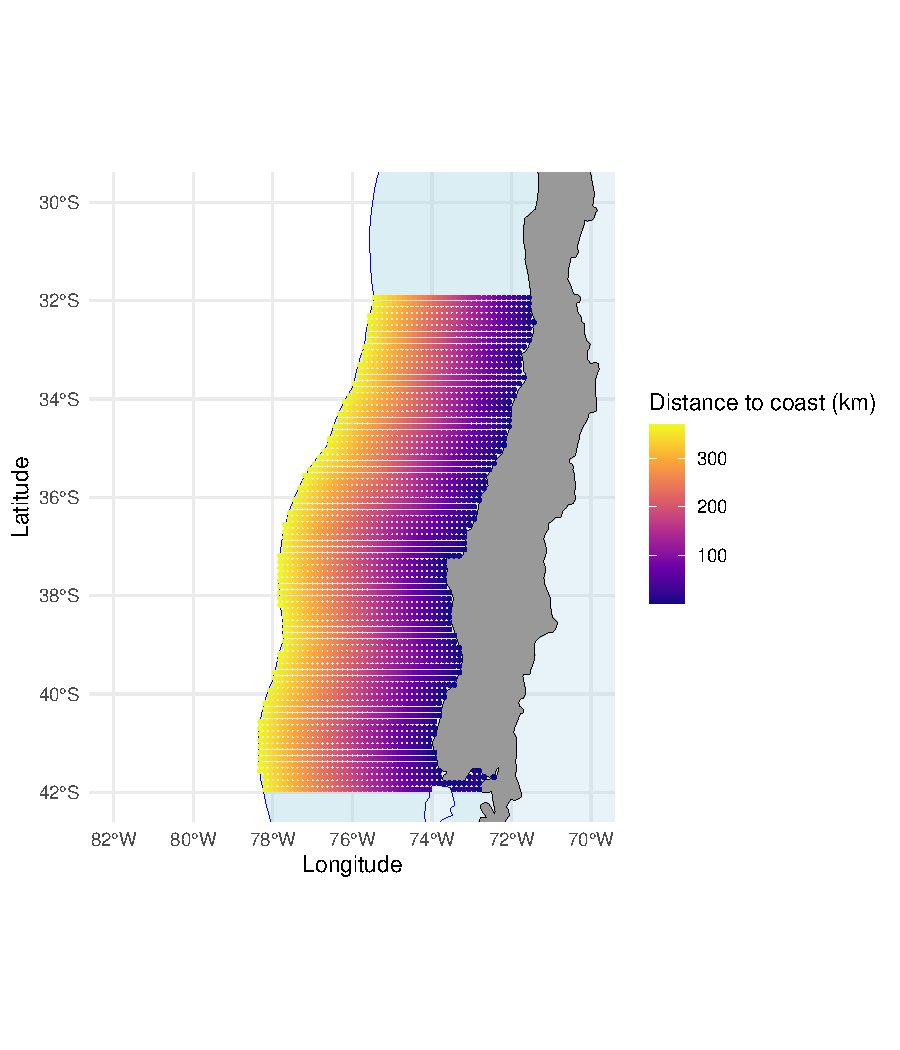
\includegraphics[width=0.8\linewidth]{../figs/env_data_map} 

}

\caption{Geographical extent of the study area used for environmental covariates limited to the Chilean Exclusive Economic Zone}\label{fig:figEnvData}
\end{figure}

\subsection{Future climate data}\label{future-climate-data}

Climate projections for SST, chlorophyll-a, and near-surface wind speed are obtained from the CMIP6 archive using a six-model ensemble selected to span the range of warming responses across the CMIP6 archive (from low- to high-sensitivity models). We use monthly outputs for two future scenarios: SSP2-4.5 (moderate) and SSP5-8.5 (high emissions). Section \emph{\nameref{projection-approach}} describes the projection horizons, baseline period, and change-factor procedure used to translate CMIP6 outputs into our empirical models.

\subsection{Econometric models}\label{econometric-models}

\subsubsection{Stock dynamics}\label{sec:stock-dynamics}

Figure \ref{fig:biomass} shows that anchoveta, sardine, and jack mackerel exhibit distinct biomass trajectories over the 2000--2024 window, with no evidence of strong interannual co-movement across species once scale differences are accounted for. Harvest pressure is visibly associated with these fluctuations; jack mackerel in particular experienced an abrupt decline during the late 2000s, consistent with the combined effects of intense fishing and unfavorable environmental conditions.

\begin{figure}[ht!]

{\centering 
\includegraphics{paper1_climate_projections_files/figure-latex/biomass-1} 

}

\caption{Estimated biomass of small pelagic species in Chile (2000--2024). Curves are LOESS-smoothed. The jack mackerel CS series is reconstructed from the IFOP acoustic record where available, imputed from the IFOP Northern Chile series via GLM otherwise, with linear interpolation as final fallback.}\label{fig:biomass}
\end{figure}

Our identification target in this subsection is the vector of climate semi-elasticities \((\rho^{SST}_s, \rho^{CHL}_s)\) across the three stocks \(s \in \{\text{anchoveta}, \text{sardine}, \text{jack mackerel}\}\)---the structural parameters that translate sea-surface temperature and chlorophyll-a anomalies into shifts in long-run stock productivity. We estimate them within a Bayesian state-space model where the latent biomass \(B_{s,t}\) of each stock follows a Schaefer law of motion whose intrinsic growth rate varies log-linearly with these forcings. The law of motion is

\begin{equation}
B_{s,t+1} \;=\; B_{s,t} + r_{s,t}\, B_{s,t}\!\left(1 - \frac{B_{s,t}}{K_s}\right) \;-\; C_{s,t} \;+\; \varepsilon_{s,t}, \qquad \varepsilon_{s,t} \sim \mathcal{N}\!\big(0,\, \sigma_{\text{proc},s}^2\big), \label{eq:law-of-motion}
\end{equation}

where \(r_{s,t}\) is the intrinsic growth rate (specified below), \(K_s\) is the stock-specific carrying capacity, \(C_{s,t}\) is the observed annual catch, and \(\varepsilon_{s,t}\) is the stochastic shock to recruitment with standard deviation \(\sigma_{\text{proc},s}\). The shocks are jointly distributed across species with a free \(3\times 3\) correlation matrix \(\Omega\) identified from the data, allowing ecological coupling not captured by the climate forcings (e.g., direct trophic interactions or competition for plankton).

Environmental conditions are summarized annually by sea surface temperature (SST) and chlorophyll-a concentration (CHL), averaged over the Centro-Sur region within the Chilean EEZ and lagged one year because environmental conditions affect recruitment and growth with a one-year delay, so that SST and CHL precede year-\(t\) biomass causally. The choice of these two covariates follows a large biological literature that identifies thermal regime and primary productivity as the dominant local drivers of small-pelagic dynamics in the Humboldt Current System (\citeproc{ref-Alheit2004}{Alheit and Niquen 2004}; \citeproc{ref-cahuin2009}{Cahuin et al. 2009}; \citeproc{ref-Yuxe1uxf1ez2014}{Yáñez et al. 2014}).

The climate shifter on \(r_{s,t}\) takes the log-linear form,

\begin{equation}
r_{s,t} \;=\; r_s^{0}\, \exp\!\Big(\, \rho_s^{SST}\, (SST_{t-1} - \overline{SST}) \;+\; \rho_s^{CHL}\, (\log CHL_{t-1} - \overline{\log CHL}) \,\Big), \label{eq:shifter}
\end{equation}

so \(\rho_s^{SST}\) and \(\rho_s^{CHL}\) are the semi-elasticities of intrinsic stock productivity to a one-degree Celsius SST anomaly and to a one-log-point chlorophyll-a anomaly \(\log(CHL_{t-1}/\overline{CHL})\), respectively. Because these parameters enter the law of motion as coefficients on exogenous climate forcings, they are generalisable---in the structural sense---to climate regimes outside the 2000--2024 estimation sample. This generalisability matters because the comparative-statics exercise of Section \emph{\nameref{projections}} applies the shifter at projected SST anomalies several SDs beyond anything observed in 2000--2024.

Latent biomass is linked to the official survey-based estimates of total stock biomass \(B_{s,t}^{\text{obs}}\) published by IFOP for all three species in Centro-Sur Chile, through a log-normal equation,

\begin{equation}
\log B_{s,t}^{\text{obs}} \;=\; \log B_{s,t} \,+\, u_{s,t}, \qquad u_{s,t} \sim \mathcal{N}\!\big(0,\, \sigma_{\text{obs},s}^2\big). \label{eq:obs}
\end{equation}

where \(u_{s,t}\) is the log-observation error---capturing sampling and detection noise in the hydroacoustic survey---with standard deviation \(\sigma_{\text{obs},s}\).

We estimate the state-space specification by Hamiltonian Monte Carlo in Stan. With \(N=25\) annual observations per stock, joint identification of \((r^{0}_s, K_s, \rho^{SST}_s, \rho^{CHL}_s)\) requires the prior information embedded in the IFOP and SPRFMO single-species assessments; Online Appendix A documents the prior construction and shows that maximum likelihood fails without these priors. We compare three nested specifications: (i) independent stocks with no climate shifters, (ii) joint stocks via \(\Omega\) with no shifters, and (iii) joint stocks with shifters (Eq. \eqref{eq:shifter}). We adopt (iii) as our primary specification; the nested predictive comparison is reported in Online Appendix B, and convergence diagnostics in Online Appendix D.

For jack mackerel we additionally fit a specification in which the growth rate is forced by the basin-scale Niño 3.4 SST anomaly at lag 1 in place of the local SST/CHL shifters, motivated by biological evidence that the Centro-Sur stock is influenced by forcing scales broader than the local coastal upwelling regime (\citeproc{ref-Arcos2001-jq}{Arcos et al. 2001}; \citeproc{ref-Pena-Torres2017-gn}{Peña-Torres et al. 2017}). The posterior of that ENSO shifter is reported in Table \ref{tab:rho-posteriors} alongside the local shifters and discussed in Online Appendix E.4; anchoveta and sardine are not refit.

\subsubsection{Total annual trips}\label{total-annual-trips}

We model the annual number of fishing trips taken by vessel \(v\) in year \(y\) as a count process following Kasperski (\citeproc{ref-Kasperski2015-jm}{2015}). We estimate separate effort models for the industrial and artisanal fleets to allow distinct elasticities to prices, allocated quota, weather, and biological closures. This specification explicitly accommodates technological heterogeneity across fleet segments, reflecting differences in vessel capacity, operating scale, and production technology.

The trip equation is a negative binomial (NB) count model:

\begin{equation}
T_{vy} \sim \text{NB}(\lambda_{vy}, \theta), \qquad \lambda_{vy} = \exp\!\left(U_{vy}'\beta\right), \label{eq:nb_trips}
\end{equation}

where \(T_{vy}\) denotes the total number of purse-seine trips recorded for vessel \(v\) in year \(y\) and \(\theta\) is the dispersion parameter that accommodates the substantial overdispersion of \(T_{vy}\) (variance-to-mean ratio of \(22.4\) for artisanal and \(4.9\) for industrial).

The vector of explanatory variables \(U_{vy}\) includes output prices by species, vessel-level allocated harvest, fixed vessel characteristics, and operating conditions:

\begin{equation}
U_{vy}=\big[p_{sy},\, H^{alloc}_{vy,s},\, Z_v,\, O_{vy}\big] \quad\text{for } s \in \{\text{anchoveta}, \text{sardine}, \text{jack mackerel}\}. \label{eq:U_trips}
\end{equation}

Output prices \(p_{sy}\) are species-specific ex-vessel prices constructed from IFOP's \emph{Monitoreo Económico de la Industria Pesquera y Acuícola Nacional} by aggregating the monthly plant-level series to annual averages over peak fishing months, following Dresdner et al. (\citeproc{ref-dresdner2013}{2013}), and deflating to constant 2018 pesos using the consumer price index from the Central Bank of Chile. Prices are mapped to each vessel through its modal departure region.

Quota shares do not enter Eq. \eqref{eq:nb_trips} directly. Instead, shares translate annual TACs into vessel-level allocated harvests. Let \(\omega_{vs}^r\) denote vessel \(v\)'s historical share of landings of species \(s\) within its administrative region \(r\) (for artisanal vessels) or regulatory zone (for industrial vessels), computed over the full sample period. Given the effective TAC \(\bar{Q}_{sy}^r\) for species \(s\) in year \(y\) and region \(r\)---obtained from SERNAPESCA quota monitoring records and reflecting all inter-fleet transfers and adjustments---vessel-level allocated harvest is:

\begin{equation}
H^{alloc}_{vy,s}=\omega_{vs}^r\,\bar{Q}_{sy}^r. \label{eq:Halloc}
\end{equation}

Each vessel is assigned to its administrative region based on its modal departure port in the logbook records. Artisanal TACs are assigned at the regional level (Valparaíso, Biobío, Araucanía, Los Ríos, Los Lagos), while industrial TACs follow the regulatory zone structure established by SUBPESCA (the Valparaíso--Araucanía and Los Ríos--Los Lagos zones for jack mackerel; the Valparaíso--Los Lagos zone for sardine and anchoveta). This regional construction introduces cross-sectional variation in \(H^{alloc}_{vy,s}\) that reflects the heterogeneous quota environments faced by vessels operating in different parts of the Centro-Sur fishery.

The vector \(Z_v\) contains time-invariant vessel characteristics, including hold capacity (log of cubic meters) and vessel type. Hold capacity determines the physical constraint on catch per trip and proxies for vessel scale.

For the artisanal fleet, preliminary diagnostics revealed within-fleet heterogeneity in the responses to both allocated anchoveta and allocated sardine: vessel-type categories differ in both the sign and magnitude of these elasticities. We therefore include \(H^{alloc}_{vy,\text{anchoveta}} \times \text{Vessel type}\) and \(H^{alloc}_{vy,\text{sardine}} \times \text{Vessel type}\) in the artisanal specification. The estimation is restricted to Vessel type categories with at least \(50\) vessel-year observations (BM, LM, UNK); smaller categories (collectively \(<0.1\%\) of artisanal effort) are excluded from the fit. The jack mackerel quota does not display this within-fleet heterogeneity.

The vector \(O_{vy}\) captures operating and regulatory constraints that vary across both vessels and years. Unlike the environmental variables in the stock dynamics model, which reflect biological productivity (SST, chlorophyll-a), the variables in the trip equation capture conditions that affect the \emph{feasibility} of fishing operations. Two vessel--year variables are constructed using each vessel's center of gravity (COG)---the catch-weighted centroid of its haul locations over the sample period. First, the number of bad-weather days is computed as the count of days per year in which the maximum daily wind speed exceeds 8 m/s at the environmental grid point (\(0.125° \approx 14\)\textasciitilde km resolution) nearest to the vessel's COG.\footnote{The wind threshold of 8 m/s corresponds approximately to Beaufort scale 5, at which purse-seine operations become difficult for artisanal vessels. We selected this threshold via AIC comparison across 8, 10, and 12 m/s cut-offs on the trip-equation fit.} Second, the number of days closed for biological closures (\textit{vedas}) is assigned based on the regulatory zone corresponding to the vessel's COG latitude. In the Centro-Sur region, sardine and anchoveta face seasonal closures for reproduction (August--October in Valparaíso--Biobío; July--October in Araucanía--Los Lagos) and recruitment (January--February in all regions), yielding 151 and 182 closed days per year, respectively. Jack mackerel has no biological closures.

Trips, harvest, and prices may be jointly determined within the year, implying potential endogeneity in reduced-form trip regressions. The purpose of Eq. \eqref{eq:nb_trips}, however, is not causal identification but rather to provide an empirically grounded behavioral relationship that maps changes in prices, quotas, and environmental conditions into expected fishing effort under projected climate scenarios.

\subsection{Projection approach}\label{projection-approach}

We assess the impact of climate change through two channels: a \emph{direct weather channel}, operating through projected changes in wind speed and the resulting number of bad-weather days; and an \emph{indirect biomass channel}, operating through projected changes in SST and CHL that modify each stock's intrinsic productivity in Eq. \eqref{eq:shifter}. Both channels ultimately enter the negative binomial trip equation. The paragraphs below describe each one and the summary statistics used to report the resulting projections.

Climate projections are derived from the six-model CMIP6 ensemble described in Section \emph{\nameref{future-climate-data}}, under SSP\(2\)-\(4.5\) and SSP\(5\)-\(8.5\). We apply the change-factor method (\citeproc{ref-Wilby2004}{Wilby et al. 2004}; \citeproc{ref-Tabor2010}{Tabor and Williams 2010}) independently to each model, preserving observed interannual variability and fine-scale spatial structure from satellite records while imposing the CMIP6 climate-change signal. For each model and variable, the delta is computed between the future climatology and a historical baseline matched to the 2000--2024 estimation window. Because CMIP6 `historical' simulations terminate in 2014, we extend the baseline through 2024 using SSP2-4.5 (near-term scenarios diverge negligibly).\footnote{One model--variable combination is spliced from SSP5-8.5 instead because the SSP2-4.5 file is missing from the model's archive.} We consider mid-century (\(2041\)--\(2060\)) and end-of-century (\(2081\)--\(2100\)) windows. The projections propagate two sources of uncertainty: (i) estimation uncertainty in the empirical parameters---the Bayesian posterior of the climate shifters (\(\rho_s^{SST}\), \(\rho_s^{CHL}\)) and the maximum-likelihood standard errors of the trip-equation coefficients (\(\beta\)'s)---and (ii) climate uncertainty from the six CMIP6 models (each gives a different projected delta).

For the direct weather channel, monthly wind speed deltas from CMIP6 are applied additively to the daily wind speed observations at each vessel's centre-of-gravity (COG); the number of bad-weather days per year is then recomputed at the projected mean using the same \(8\) m/s operability threshold as in the historical panel. Because the historical daily wind distribution at vessel COGs sits sufficiently close to the threshold, a small upward shift in the mean displaces a non-negligible mass of the upper tail past it, generating substantially more days exceeding the threshold despite the small absolute change in the mean.

For the indirect biomass channel, the CMIP6 SST delta (in °C) and log-CHL delta (in log-points) are added to the historical anomaly series. These enter Eq. \eqref{eq:shifter} and shift each stock's intrinsic growth rate to \(r_s^{\star} = r_s^{0} \cdot \exp(\rho_s^{SST}\, \Delta SST + \rho_s^{CHL}\, \Delta \log CHL)\). The new \(r_s^{\star}\) translates into the Schaefer steady-state biomass \(B_s^{\star} = K_s(1 - \bar{F}_s/r_s^{\star})\), which collapses to zero whenever \(\bar{F}_s \geq r_s^{\star}\); the instantaneous fishing mortality \(\bar{F}_s\) is computed empirically as the 2000--2024 average of \(C_{s,t}/B_{s,t}\) (observed catch over observed biomass) and held fixed across scenarios (see the comparative-statics framing below). Let \(\Delta r_s^{\star}/r_s^{0} \equiv r_s^{\star}/r_s^{0} - 1\) denote the resulting long-run productivity shift.

Because \(\Delta r_s^{\star}/r_s^{0}\) is a random variable over both dimensions (the six CMIP6 models and the posterior of the shifters), we report four summary statistics that separate the corresponding two sources of uncertainty. \emph{Climate uncertainty}---the contribution of disagreement across CMIP6 models---is summarised by computing the within-model posterior median of \(\Delta r_s^{\star}/r_s^{0}\) for each of the six models and then reporting the median and IQR across those six model-specific medians. \emph{Structural uncertainty}---the contribution of parameter uncertainty about the shifters---is summarised by evaluating \(\Delta r_s^{\star}/r_s^{0}\) at every posterior draw conditional on each CMIP6 model, taking the 5th and 95th percentiles to form a within-model 90\% posterior credible interval, and reporting the median lower bound and median upper bound across the six models. Finally, we report the posterior probability of a negative impact, \(\Pr(\Delta r_s^{\star}/r_s^{0} < 0)\), computed within each CMIP6 model as the fraction of posterior draws yielding a negative shift and then taken as the cross-model median.

The fleet-level effort response combines both projection channels in the trip equation. Under proportional-TAC management, each species-specific biomass shift \(B_s^{\star}/B_s^{0}\) scales the corresponding \(H^{alloc}_{vy,s}\); the projected number of \emph{Bad weather days} (recomputed from the CMIP6 wind delta, as described above) replaces the historical value of the same variable used in the trip equation. Each vessel's projected \(T_v^{\star}\) therefore reflects all three biomass shifts simultaneously---weighted by its historical exposure to each species---plus the direct weather shock. Any stock whose climate shifters fail to identify in the historical fit has its biomass shift fixed at \(B_s^{\star}/B_s^{0}=1\) in the projection; in this paper, this rule applies to jack mackerel (see Section \emph{\nameref{identification}}).

To diagnose how much of the projected trip response is driven by full portfolio collapse versus by gradual climate elasticities, we construct a single \emph{composition-weighted biomass factor} per vessel,
\begin{equation}
f^H_v \;=\; \sum_s \omega_{vs}\,\frac{B_s^{\star}}{B_s^{0}}, \label{eq:fHv}
\end{equation}
where \(\omega_{vs}\) is vessel \(v\)'s realised catch share in species \(s\) over the historical sample. The factor \(f^H_v\) does not enter the trip equation as a regressor; it is a derived statistic of each posterior draw, used as a threshold for the conditional median and as the basis for \(\Pr(f^H_v<0.5)\). We summarise the fleet-level percentage change in trips, \(\%\Delta T_f\), with two posterior medians: the \emph{marginal} median integrates over all posterior draws within each model and captures the full response (including portfolio collapse); the \emph{conditional} median restricts the integration to draws with \(f^H_v \geq 0.5\), isolating the pure climate-elasticity component from the steady-state collapse component. We also report the posterior probability of portfolio loss, \(\Pr(f^H_v<0.5)\), as a stand-alone measure of collapse risk. All three statistics are aggregated across CMIP6 models via cross-model median and IQR, in parallel with the productivity statistics above.

Our framework is positioned as long-run comparative statics, not a year-by-year forecast. Because the empirical models are estimated on interannual variability rather than decadal trends, the projections capture short-run behavioural responses to environmental and weather shocks but cannot identify long-run adaptation by fishers or managers (\citeproc{ref-Aufhammer2018}{Auffhammer 2018}). Prices, quotas, and adaptive behaviour are held fixed at historical levels. The framework therefore provides a benchmark for the direction and magnitude of climate impacts under a fixed-institution baseline; relaxations that endogenize price adjustment, quota revision, or vessel-level adaptation are flagged as natural extensions of this work.

\section{Results}\label{results}

\subsection{Identification of climate shifters}\label{identification}

Table \ref{tab:rho-posteriors} reports the posterior identification of
the local climate shifters \(\{\rho_s^{SST}, \rho_s^{CHL}\}_{s=1}^{3}\)
introduced in Section \emph{\nameref{methods}}, together with the
basin-scale ENSO shifter \(\rho^{\text{ENSO}}_{\text{jur}}\) from the
jack mackerel refit of Online Appendix E.4. The model reproduces the historical biomass trajectories within a median 90\% posterior band width of approximately 20\% of the mean; posterior-predictive and convergence diagnostics are reported in Online Appendices C and D. Priors are weakly informative
and elicited from IFOP and SPRFMO single-species assessments (Appendix A). The
posterior-to-prior standard-deviation ratio in the rightmost column
measures how much the 2000--2024 biomass series refines each parameter
relative to the prior; values well below one indicate identification from
the likelihood.\footnote{The ratio captures the relative information content of the data, isolating identification from prior centring: a precise likelihood shrinks the posterior dispersion around wherever the data locate the parameter, whereas a non-informative likelihood leaves the prior dispersion unchanged regardless of how the posterior mean moves.}

\begin{table}[!h]
\centering
\caption{\label{tab:rho-posterior-table}Posterior identification of climate shifters. \label{tab:rho-posteriors}}
\centering
\fontsize{10}{12}\selectfont
\begin{threeparttable}
\begin{tabular}[t]{llcccrr}
\toprule
Shifter & Stock & Prior $\mathcal{N}(\mu, \sigma)$ & Posterior mean & Posterior 90\% CI & $\sigma_{\text{post}}/\sigma_{\text{prior}}$ & $\hat{R}$\\
\midrule
$\rho^{SST}$ & Anchoveta CS & $\mathcal{N}(-2.3, 1.0)$ & -1.06 & {}[-1.79, -0.38] & 0.43 & 1.000\\
$\rho^{SST}$ & Sardine CS & $\mathcal{N}(-2.0, 1.0)$ & -2.75 & {}[-3.46, -2.02] & 0.44 & 1.000\\
$\rho^{SST}$ & Jack mackerel CS & $\mathcal{N}(0.0, 1.0)$ & 0.42 & {}[-1.25, 2.09] & 1.01 & 1.000\\
$\rho^{CHL}$ & Anchoveta CS & $\mathcal{N}(-2.3, 1.0)$ & -3.64 & {}[-5.01, -2.25] & 0.83 & 1.000\\
$\rho^{CHL}$ & Sardine CS & $\mathcal{N}(2.1, 1.0)$ & 2.17 & {}[0.96, 3.37] & 0.74 & 1.000\\
\addlinespace
$\rho^{CHL}$ & Jack mackerel CS & $\mathcal{N}(0.0, 1.0)$ & -0.06 & {}[-1.72, 1.60] & 1.01 & 1.001\\
$\rho^{ENSO}$ & Jack mackerel CS & $\mathcal{N}(0.0, 0.5)$ & -0.02 & {}[-0.81, 0.80] & 0.98 & 1.000\\
\bottomrule
\end{tabular}
\begin{tablenotes}
\item \textit{Note:} 
\item Shifters are semi-elasticities of intrinsic growth $r_s$ with respect to local SST (°C), local log-CHL (log-points), and the basin-scale Niño 3.4 index. The ENSO row reports the lag-1 refit of Online Appendix E.4 for jack mackerel only; anchoveta and sardine inherit their main-specification posteriors. All $\hat{R} \leq 1.01$.
\end{tablenotes}
\end{threeparttable}
\end{table}

Three patterns in Table \ref{tab:rho-posteriors} organise the
discussion: (i) the two coastal stocks are identified on both shifters,
with sardine's SST semi-elasticity roughly twice that of anchoveta; (ii) their CHL
shifters carry opposite signs; and (iii)
jack mackerel returns a structural null on all three shifters, including the basin-scale ENSO refit.

First, for the two coastal upwelling stocks---anchoveta and sardine
común---both climate shifters are identified with substantial precision.
The posterior 90\% credible intervals exclude zero for all four parameters,
and the standard deviation ratios fall between \(0.43\) and \(0.83\),
indicating that the 2000--2024 biomass series refines the priors
materially. For anchoveta, a one-degree positive SST anomaly is associated
with a semi-elasticity of \(\rho^{SST}_{\text{anch}} = -1.06\)
(CI \([-1.79, -0.38]\)); for sardine, the corresponding semi-elasticity
is more than twice as large, \(\rho^{SST}_{\text{sard}} = -2.75\)
(CI \([-3.46, -2.02]\)). Both signs are consistent with the regional literature: the negative SST sensitivity for anchoveta aligns with the cold-water anchovy regime documented for the Humboldt Current ecosystem (\citeproc{ref-Alheit2004}{Alheit and Niquen 2004}; \citeproc{ref-Schwartzlose1999-uy}{Schwartzlose et al. 1999}), and the stronger sardine sensitivity matches the negative coupling between SST anomalies and \emph{Strangomera bentincki} recruitment in Centro-Sur Chile reported by Gomez et al. (\citeproc{ref-Gomez2012}{2012}) with \(r=-0.83\). Evaluated at one historical standard deviation of
the SST anomaly series (estimation-sample \(\hat{\sigma}_{SST} =
0.26\,^{\circ}\text{C}\) over 2000--2024), a thermal shock of that magnitude
lowers the intrinsic growth rate of anchoveta by approximately 24\%
(\(1 - e^{-1.06 \cdot 0.26}\)) and that of sardine by approximately 51\%
(\(1 - e^{-2.75 \cdot 0.26}\)) relative to the climatological mean. Under a
policy-relevant warming signal of \(+1\,^{\circ}\text{C}\), comparable to
mid-century CMIP6 SSP2-4.5 projections for the Chilean coastal zone, the
implied declines are 65\% for anchoveta and 94\% for sardine. Applied
to a fishery whose anchoveta--sardine combined
Centro-Sur TAC has averaged roughly \(440\) kt per year over the 2012--2024
window, the implied losses are on the order of \(300\)--\(400\) kt per year
under sustained \(+1\,^{\circ}\text{C}\) warming. The caveat is that
\(+1\,^{\circ}\text{C}\) lies approximately four historical standard
deviations beyond the 2000--2024 estimation window, so the projection
relies on the log-linear extrapolation embedded in the shifter function.

Second, the two coastal stocks respond to chlorophyll-a with opposite signs: \(\rho^{CHL}_{\text{anch}} = -3.64\) (CI \([-5.01, -2.25]\)) versus
\(\rho^{CHL}_{\text{sard}} = +2.17\) (CI \([+0.96, +3.37]\)). At one historical
standard deviation of \(\log CHL\) (\(\hat{\sigma}_{\log CHL} = 0.095\), a
primary-productivity anomaly of roughly 10\%), a positive CHL shock lowers
anchoveta growth by approximately 29\% while raising sardine growth by
approximately 23\%. The opposite-signed CHL semi-elasticities in Table \ref{tab:rho-posteriors} are consistent with the well-documented anchoveta--sardine asymmetry under regime shifts in the Humboldt Current ecosystem (\citeproc{ref-Alheit2004}{Alheit and Niquen 2004}; \citeproc{ref-Schwartzlose1999-uy}{Schwartzlose et al. 1999}): they might reflect the relative competitive dynamics between the two species under high-productivity regimes rather than a direct biological effect of chlorophyll on anchoveta. The positive coupling between coastal chlorophyll and common sardine recruitment in Centro-Sur Chile is documented with correlation \(r=0.92\) between CHL and log recruitment by Gomez et al. (\citeproc{ref-Gomez2012}{2012}). A warming-and-greening regime
therefore does not produce a uniform shock on the artisanal fleet,
because anchoveta and sardine respond to chlorophyll with opposite signs.
The net impact on each vessel depends on its realized catch composition
over the two species, which we integrate at the fleet level in Section
\emph{\nameref{projections}}.

Third, and in marked contrast, neither SST nor CHL shifters are identified for jack mackerel. Unlike anchoveta and sardine, jack mackerel priors are vague and centered at zero (Appendix A), so the posterior moves only if the data refines it. That the posterior coincides with the prior---\(\sigma_{\text{post}}/\sigma_{\text{prior}} \approx 1\), means near zero, credible intervals straddling zero---indicates that the 2000--2024 biomass series provides insufficient information to identify climate effects on jack mackerel productivity at this scale, consistent with jack mackerel ranging across the broader Southeast Pacific rather than being driven by local Chilean conditions (it is managed through SPRFMO accordingly). The model correctly reports this non-identification rather than producing a spurious coefficient.

Online Appendix E reports five complementary robustness tests of this null: three nested coastal aggregations, a dual-source extension with a Northern Chilean acoustic series, basin-scale ENSO shifters at lags 1 and 2, a joint specification with all three shifters active simultaneously, and an extension using the broader SPRFMO range-wide jack mackerel stock assessment. All five converge on posterior-to-prior ratios between \(0.94\) and \(1.03\), indistinguishable from unity. These tests try to rule out the standard technical explanations for the null: too small an area, too few years, the wrong climate variable, the wrong econometric specification, or the wrong geographic scope. The relevant climate forcing for the Centro-Sur jack mackerel stock operates at margins---behaviour, location, and the seasonal timing of spawning and migration (\citeproc{ref-Arancibia2019-FIPA}{Arancibia et al. 2019}; \citeproc{ref-Arcos2001-jq}{Arcos et al. 2001}; \citeproc{ref-Pena-Torres2017-gn}{Peña-Torres et al. 2017})---not captured in the elasticity of annual aggregate productivity.

Figure \ref{fig:rho-forest} visualises the posterior--prior updating as a
forest plot.

\begin{figure}[!htbp]
\centering
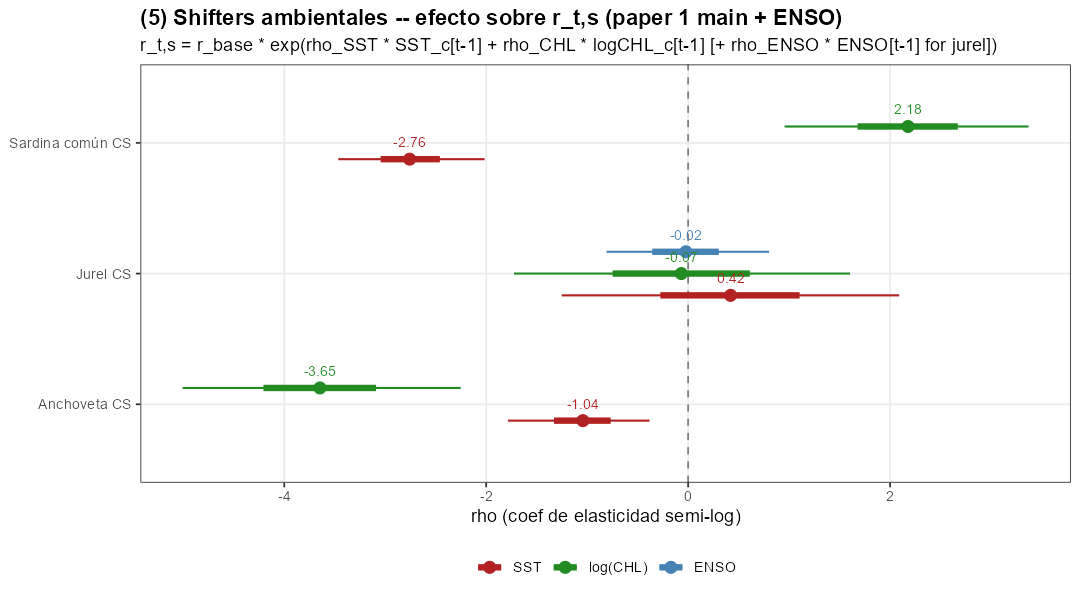
\includegraphics[width=0.75\textwidth]{../figs/t4b/t4b_full_rho_shifters.png}
\caption{Posterior and prior distributions of the climate shifters $\rho_s^{SST}$, $\rho_s^{CHL}$, and $\rho_{jur}^{ENSO}$ by stock. Solid lines show the posterior $90\%$ (thin) and $50\%$ (thick) credible intervals; dashed lines show the prior $90\%$ credible interval. Anchoveta and sardine show substantial posterior updating with narrow credible intervals excluding zero. Jack mackerel posteriors (SST, CHL, ENSO) coincide with their vague priors centred at zero, indicating non-identification.}
\label{fig:rho-forest}
\end{figure}

\subsection{Total annual trips}\label{sec:tripresults}

Table \ref{tab:poisson_results} reports the negative binomial estimates separately for each fleet segment. The specification includes year fixed effects, which absorb aggregate shocks affecting both fleets contemporaneously---most notably the 2019 social outbreak (\emph{estallido social}) and the 2020--2022 COVID-19 period---and identify the trip-equation coefficients from within-year cross-vessel variation.

\begin{table}[!ht] \centering 
  \caption{Negative binomial estimates of annual fishing trips (2013--2024, $N_{IND}$ = 319, $N_{ART}$ = 4184)} 
  \label{tab:poisson_results} 
\footnotesize 
\begin{threeparttable}
\begin{tabular}{@{\extracolsep{5pt}}lcc} 
\\[-1.8ex]\hline 
\hline \\[-1.8ex] 
 & \multicolumn{2}{c}{\textit{Dependent variable:}} \\ 
\cline{2-3} 
 & Industrial & Artisanal \\ 
\\[-1.8ex] & (1) & (2)\\ 
\hline \\[-1.8ex] 
 Hold capacity (log m$^3$) & 0.097 (0.221) & 0.132$^{***}$ (0.045) \\ 
  Allocated harvest anchoveta ($H^{alloc}_{vy,anch}$, tons) & $-$0.0003 (0.0002) & 0.007$^{***}$ (0.002) \\ 
  Allocated harvest sardine ($H^{alloc}_{vy,sard}$, tons) & 0.0001$^{***}$ (0.00003) & 0.004$^{***}$ (0.001) \\ 
  Allocated harvest jack mackerel ($H^{alloc}_{vy,jur}$, tons) & 0.00002$^{*}$ (0.00001) & 0.001 (0.0005) \\ 
  Price anchoveta (1000s \$/ton) & $-$0.004 (0.004) & 0.010$^{***}$ (0.003) \\ 
  Price sardine (1000s \$/ton) & $-$0.016$^{***}$ (0.003) & 0.004$^{**}$ (0.002) \\ 
  Price jack mackerel (1000s \$/ton) & 0.008$^{***}$ (0.003) & 0.007$^{***}$ (0.002) \\ 
  Bad weather days & $-$0.0003 (0.001) & $-$0.001 (0.0005) \\ 
  Veda days & $-$0.079$^{***}$ (0.005) & 0.012$^{***}$ (0.002) \\ 
  Vessel type (UNK) & $-$1.450$^{***}$ (0.163) & 0.166 (0.102) \\ 
  Vessel type (LM) &  & 0.466$^{***}$ (0.100) \\ 
  $H^{alloc}_{vy,anch} \times$ Vessel type (LM) &  & $-$0.007$^{***}$ (0.002) \\ 
  $H^{alloc}_{vy,anch} \times$ Vessel type (UNK) &  & $-$0.007$^{***}$ (0.002) \\ 
  $H^{alloc}_{vy,sard} \times$ Vessel type (LM) &  & $-$0.003$^{***}$ (0.001) \\ 
  $H^{alloc}_{vy,sard} \times$ Vessel type (UNK) &  & $-$0.00002 (0.001) \\ 
  Constant & 15.763$^{***}$ (2.605) & $-$3.776$^{***}$ (0.519) \\ 
 \hline \\[-1.8ex] 
Year fixed effects & Yes & Yes \\ 
Pseudo-$R^2$ (Cragg-Uhler) & 0.302 & 0.632 \\ 
Observations & 319 & 4,184 \\ 
\hline 
\hline \\[-1.8ex] 
\end{tabular}
\begin{tablenotes}[flushleft]
\footnotesize
\item \textit{Note:} $^{*}$p$<$0.1; $^{**}$p$<$0.05; $^{***}$p$<$0.01. Vessel-clustered robust SEs. Prices in constant 2018 thousands of pesos/ton.
\item LR test NB vs Poisson: Industrial $\chi^2$ = 397.6; Artisanal $\chi^2$ = 36496.9 (both $p < 0.001$).
\end{tablenotes}
\end{threeparttable}
\end{table}

The coefficients on species-specific allocated harvest reveal cross-fleet heterogeneity. For the industrial fleet, the sardine allocation yields a positive and significant trip response (\(p < 0.001\)), the jack mackerel allocation is positive and marginally significant (\(p < 0.10\)), and the anchoveta coefficient is not statistically distinguishable from zero. The artisanal fleet shows positive and significant responses to anchoveta and sardine allocations (both at \(p < 0.001\)); the jack mackerel allocation is positive but not statistically distinguishable from zero. Both species show scale-dependent responses in the artisanal fleet, but with different patterns. For anchoveta, only the \emph{bote motor} (BM, \(8\%\) of the panel) exhibits a positive marginal coefficient (\(\hat{\beta}_h^{\,\mathrm{anch,BM}} = +0.007\), \(p < 0.01\)); the \emph{lancha motor} (LM, \(77\%\)) and \emph{unidentified} (UNK, \(14\%\)) categories cancel this base effect through significant negative interactions (\(-0.007\) each, both \(p < 0.01\)). For sardine, BM and UNK exhibit positive coefficients (\(\hat{\beta}_h^{\,\mathrm{sard,BM}} = +0.004\), \(p < 0.01\); UNK interaction \(\approx 0\)); only LM cancels the base effect through a significant negative interaction (\(-0.003\), \(p < 0.01\)).

The two fleets differ in price responsiveness. For the industrial fleet, both the jack mackerel and sardine prices are significant at the 1\% level---jack mackerel with a positive coefficient and sardine with a negative coefficient; the anchoveta price has no detectable effect. The artisanal fleet shows positive and significant coefficients on all three prices: anchoveta and jack mackerel at the 1\% level and sardine at the 5\% level. The artisanal pattern is consistent with a standard supply-side response: higher ex-vessel prices for the species the fleet targets are associated with more trips. The negative industrial sardine-price coefficient is contrary to a supply response, but the trip equation is not a causal demand specification---prices, harvest allocations, and biomass are jointly determined within the panel---and prices enter only as control variables that absorb year-on-year market variation.

Hold capacity is not significant for the industrial fleet, where vessels are relatively homogeneous in scale, but it is positive and significant for the artisanal fleet. Among artisanal vessels, larger hold capacity is associated with more annual trips, consistent with larger vessels being more commercially active and better able to sustain operations across varying conditions.

The environmental and regulatory variables show distinct patterns. Adverse weather days carry a negative coefficient for both fleets but are not statistically distinguishable from zero. We retain these point estimates for the direct weather channel of Section \emph{\nameref{projection-approach}}; their estimation uncertainty propagates into the cross-model spread of Table \ref{tab:trip_compstat}. Biological closure days are strongly negative for the industrial fleet. The artisanal coefficient is positive but admits no causal reading under year fixed effects: the underlying closure variable is constant within each artisanal management zone, so the regression identifies only off the cross-zone differential and conflates locational heterogeneity in artisanal effort intensity with the causal effect of closures.

\subsection{Climate change projections}\label{projections}

The projection methodology is summarized in Section \emph{\nameref{projection-approach}}. Under each scenario and time window, we translate CMIP6-derived environmental deltas into (i) changes in bad-weather days that enter the trip equation (direct channel) and (ii) posterior draws of the stock-specific effective growth rate \(r_{s,t}^{\star}\), obtained by evaluating the identified climate shifter of Eq. \eqref{eq:shifter} at the projected SST and log-CHL anomalies (indirect channel).

\subsubsection{Projected environmental changes}\label{projected-environmental-changes}

Table \ref{tab:env_projections} summarises the projected environmental changes as cross-model medians with cross-model interquartile range (IQR). SST warms by \(+0.6\) to \(+2.4\,^{\circ}\)C across scenarios. The chlorophyll-a cross-model median is close to zero in all scenario-window pairs (between \(-1.3\%\) and \(+2.2\%\)), while the cross-model IQR is substantially wider (up to \(-7\%\) to \(+3\%\) under SSP5-8.5 end-of-century), reflecting documented CMIP6 disagreement on primary-productivity responses. Wind speed increases modestly (\(+0.1\) to \(+0.4\) m/s cross-model median), but translates into \(+8.5\) to \(+23.5\) additional bad-weather days per year because the historical daily wind distribution at vessel COGs sits sufficiently close to the 8 m/s operability threshold that a small upward shift in the mean displaces a non-negligible mass of the upper tail past it.

\begin{table}[!h]
\centering
\caption{\label{tab:envprojections}Projected environmental changes for Centro-Sur Chile (CMIP6 ensemble, change-factor method; cross-model median with cross-model IQR in brackets). \label{tab:env_projections}}
\centering
\begin{threeparttable}
\fontsize{9}{11}\selectfont
\begin{tabular}[t]{llrlll}
\toprule
SSP & Window & $n_m$ & $\Delta$ SST ($^{\circ}$C) & $\Delta$ CHL (\%) & $\Delta$ wind speed (m/s)\\
\midrule
SSP2-4.5 & 2081--2100 & 5 & $+1.31$ \,[$+0.84$, $+1.56$] & $+0.0$ \,[$-3.6$, $+1.4$] & $+0.19$ \,[$+0.10$, $+0.24$]\\
SSP2-4.5 & 2041--2060 & 5 & $+0.58$ \,[$+0.50$, $+0.93$] & $+2.2$ \,[$+0.0$, $+2.8$] & $+0.14$ \,[$+0.13$, $+0.15$]\\
SSP5-8.5 & 2081--2100 & 6 & $+2.39$ \,[$+1.93$, $+3.29$] & $-1.3$ \,[$-7.4$, $+3.0$] & $+0.42$ \,[$+0.36$, $+0.45$]\\
SSP5-8.5 & 2041--2060 & 6 & $+0.92$ \,[$+0.61$, $+1.23$] & $+0.7$ \,[$-2.3$, $+3.4$] & $+0.21$ \,[$+0.14$, $+0.32$]\\
\bottomrule
\end{tabular}
\begin{tablenotes}
\item \textit{Note:} 
\item SSP2-4.5 panels use 5 instead of 6 CMIP6 models because one model does not publish chlorophyll-a projections for that scenario.
\end{tablenotes}
\end{threeparttable}
\end{table}

\subsubsection{Comparative statics on intrinsic stock productivity}\label{comparative-statics-on-intrinsic-stock-productivity}

Table \ref{tab:growth_compstat} reports the four summary statistics of \(\Delta r_s^{\star}/r_s^{0}\) defined in Section \emph{\nameref{projection-approach}}, for each stock under each scenario-window pair. Jack mackerel is reported as non-identified (``n.i.'\,') consistent with the identification result in Section \emph{\nameref{identification}}.

Under the moderate SSP2-4.5 mid-century scenario (cross-model median \(+0.58\,^{\circ}\)C; \(\Delta\log\text{CHL}\) near zero in the cross-model median, with non-trivial cross-model spread), the cross-model median of anchoveta's intrinsic productivity declines by \(51\%\) and sardine's by \(79\%\), with posterior probability of negative impact equal to one in both cases.

Under the high-emissions SSP5-8.5 end-of-century scenario (cross-model median \(+2.39\,^{\circ}\)C, \(\Delta\log\text{CHL}\) cross-model median \(-0.013\) with \(5\)th-percentile of \(-0.30\) across models) the cross-model medians deepen to \(-90\%\) and \(-99.9\%\) respectively, and the entire \(90\%\) credible interval of sardine's response lies below zero in every model of the ensemble. The anchoveta cross-model probability of decline is \(0.99\) rather than \(1\) because under a small fraction of (model, draw) pairs a sufficiently negative \(\Delta\log\text{CHL}\) combined with \(\rho^{CHL}_{\text{anch}}<0\) offsets the SST-driven collapse.

The identified signs confirm the qualitative reading of the shifters in Section \emph{\nameref{identification}}: both coastal stocks respond negatively to SST, but sardine carries roughly twice the SST semi-elasticity of anchoveta, and its CHL semi-elasticity is of the opposite sign, so that the compound response---negative thermal shock combined with negative primary-productivity shock---is sharper for sardine than for anchoveta.

\begin{landscape}
\begin{table}[!h]
\centering
\caption{\label{tab:growthcompstat}Comparative statics on intrinsic stock productivity under the CMIP6 six-model ensemble. \label{tab:growth_compstat}}
\centering
\resizebox{\ifdim\width>\linewidth\linewidth\else\width\fi}{!}{
\fontsize{8}{10}\selectfont
\begin{threeparttable}
\begin{tabular}[t]{llccccccr}
\toprule
\multicolumn{5}{c}{ } & \multicolumn{4}{c}{Summary statistics} \\
\cmidrule(l{3pt}r{3pt}){6-9}
Stock & Scenario & $n_m$ & $\Delta SST$ ($^{\circ}$C) & $\Delta \log\text{CHL}$ & Cross median & Cross-model IQR & Within posterior 90\% CI & $\Pr(\Delta<0)$\\
\midrule
Anchoveta CS & SSP2-4.5, 2041-2060 & 5 & +0.58 & +0.022 & -50.7\% & {}[-52.7\%, -47.8\%] & {}[-68.0\%, -27.0\%] & 1.00\\
Anchoveta CS & SSP2-4.5, 2081-2100 & 5 & +1.31 & +0.000 & -71.0\% & {}[-76.3\%, -60.4\%] & {}[-91.1\%, -31.0\%] & 1.00\\
Anchoveta CS & SSP5-8.5, 2041-2060 & 6 & +0.92 & +0.007 & -62.4\% & {}[-68.0\%, -55.9\%] & {}[-80.9\%, -31.2\%] & 1.00\\
Anchoveta CS & SSP5-8.5, 2081-2100 & 6 & +2.39 & -0.013 & -89.6\% & {}[-91.5\%, -87.4\%] & {}[-98.3\%, -54.2\%] & 0.99\\
Sardine CS & SSP2-4.5, 2041-2060 & 5 & +0.58 & +0.022 & -78.6\% & {}[-93.2\%, -72.5\%] & {}[-85.7\%, -67.3\%] & 1.00\\
\addlinespace
Sardine CS & SSP2-4.5, 2081-2100 & 5 & +1.31 & +0.000 & -97.2\% & {}[-98.9\%, -89.8\%] & {}[-98.9\%, -92.6\%] & 1.00\\
Sardine CS & SSP5-8.5, 2041-2060 & 6 & +0.92 & +0.007 & -91.1\% & {}[-96.7\%, -78.5\%] & {}[-95.1\%, -83.2\%] & 1.00\\
Sardine CS & SSP5-8.5, 2081-2100 & 6 & +2.39 & -0.013 & -99.9\% & {}[-100.0\%, -99.4\%] & {}[-100.0\%, -99.3\%] & 1.00\\
Jack mackerel CS & SSP2-4.5, 2041-2060 & 5 & +0.58 & +0.022 & n.i. & n.i. & n.i. & n.i.\\
Jack mackerel CS & SSP2-4.5, 2081-2100 & 5 & +1.31 & +0.000 & n.i. & n.i. & n.i. & n.i.\\
\addlinespace
Jack mackerel CS & SSP5-8.5, 2041-2060 & 6 & +0.92 & +0.007 & n.i. & n.i. & n.i. & n.i.\\
Jack mackerel CS & SSP5-8.5, 2081-2100 & 6 & +2.39 & -0.013 & n.i. & n.i. & n.i. & n.i.\\
\bottomrule
\end{tabular}
\begin{tablenotes}
\item \textit{Note:} 
\item SSP2-4.5 panels use 5 instead of 6 CMIP6 models because one model does not publish chlorophyll-a projections for that scenario. Jack mackerel CS is reported as non-identified ('n.i.'); see Results identification section.
\end{tablenotes}
\end{threeparttable}}
\end{table}
\end{landscape}

The comparative-statics exercise is a long-run object rather than a year-by-year forecast. It describes the steady-state intrinsic productivity of each stock under a counterfactual climate, \emph{holding fixed} the law of motion and the fishery's regulatory regime. The shifters \((\rho_s^{SST}, \rho_s^{CHL})\) enter the law of motion as coefficients on exogenous climate forcings, which makes them invariant to the joint distribution of \((SST, B, C)\) and therefore evaluable at climate regimes outside the estimation window---in particular, at an SST anomaly of \(+2.3^{\circ}\)C that lies roughly nine historical standard deviations beyond the 2000--2024 mean. A purely correlational specification would not license this extrapolation.

\subsubsection{Implications for fleet-level effort}\label{implications-for-fleet-level-effort}

Table \ref{tab:trip_compstat} translates the productivity shifts of Table \ref{tab:growth_compstat} into projected fleet-level trips by running each posterior draw under each CMIP6 model through the projection machinery of Section \emph{\nameref{projection-approach}}. Fleet-level summary statistics follow the within-model-then-cross-model aggregation used in Table \ref{tab:growth_compstat}, but applied to the three quantities defined in Section \emph{\nameref{projection-approach}}: the marginal and conditional posterior medians of \(\%\Delta T_f\), and the posterior probability of portfolio loss, \(\Pr(f^H_v<0.5)\).

\begin{table}[!h]
\centering
\caption{\label{tab:tripcompstat}Long-run implications of CMIP6 climate scenarios for fleet-level fishing effort. Summary statistics defined in Section \emph{\nameref{projection-approach}}. \label{tab:trip_compstat}}
\centering
\fontsize{9}{11}\selectfont
\begin{threeparttable}
\begin{tabular}[t]{llcll}
\toprule
Fleet & Scenario & $\Pr(f^H_v < 0.5)$ & $\%\Delta$ trips (marginal) & $\%\Delta$ trips (conditional)\\
\midrule
Artisanal & SSP2-4.5, 2041-2060 & 0.95\,[0.93,\,0.96] & -16.1\%\,[-16.9\%,\,-14.9\%] & -8.0\%\,[-8.2\%,\,-7.7\%]\\
Artisanal & SSP2-4.5, 2081-2100 & 0.98\,[0.97,\,0.99] & -17.0\%\,[-17.1\%,\,-16.9\%] & -7.9\%\,[-13.8\%,\,-5.2\%]\\
Artisanal & SSP5-8.5, 2041-2060 & 0.98\,[0.96,\,0.98] & -16.6\%\,[-16.8\%,\,-15.9\%] & -8.8\%\,[-11.2\%,\,-6.5\%]\\
Artisanal & SSP5-8.5, 2081-2100 & 0.99\,[0.99,\,0.99] & -17.6\%\,[-17.8\%,\,-17.5\%] & -6.2\%\,[-10.6\%,\,-5.9\%]\\
Industrial & SSP2-4.5, 2041-2060 & 0.12\,[0.11,\,0.12] & -1.0\%\,[-1.0\%,\,-0.8\%] & -0.7\%\,[-0.7\%,\,-0.7\%]\\
Industrial & SSP2-4.5, 2081-2100 & 0.12\,[0.12,\,0.12] & -0.9\%\,[-1.0\%,\,-0.8\%] & -0.7\%\,[-0.8\%,\,-0.7\%]\\
Industrial & SSP5-8.5, 2041-2060 & 0.12\,[0.12,\,0.12] & -0.8\%\,[-0.9\%,\,-0.8\%] & -0.7\%\,[-0.9\%,\,-0.7\%]\\
Industrial & SSP5-8.5, 2081-2100 & 0.12\,[0.12,\,0.12] & -1.0\%\,[-1.1\%,\,-1.0\%] & -1.0\%\,[-1.0\%,\,-0.9\%]\\
\bottomrule
\end{tabular}
\begin{tablenotes}
\item \textit{Note:} 
\item SSP2-4.5 panels use 5 instead of 6 CMIP6 models because one model does not publish chlorophyll-a projections for that scenario.
\end{tablenotes}
\end{threeparttable}
\end{table}

The posterior probability of portfolio loss---defined as a reduction of more than fifty percent in the composition-weighted biomass factor \(f^H_v\) relative to the 2000--2024 historical baseline---exceeds 0.95 for the artisanal fleet under every CMIP6 scenario considered and reaches 0.99 under SSP5-8.5 end-of-century. For the industrial fleet, the loss probability is a stable 0.12 across all four scenarios, driven entirely by its five-percent exposure to sardine; the remaining 95\% of its historical portfolio is allocated to jack mackerel, whose climate shifter is treated as non-identified in Section \emph{\nameref{identification}}. The asymmetry in loss probability between the two fleets is large and stable across climate pathways, approximately eight-fold across all four scenarios.

Decomposing the fleet-level trip response isolates the channels through which this asymmetry operates. The \emph{marginal} posterior median of \(\%\Delta\) trips ranges from \(-16.1\%\) (SSP2-4.5 mid) to \(-17.6\%\) (SSP5-8.5 end) for the artisanal fleet and from \(-0.8\%\) to \(-1.0\%\) for the industrial fleet---a ratio of roughly seventeen to one at end-of-century. The \emph{conditional} posterior median, restricted to draws with \(f^H_v \geq 0.5\), isolates the climate-elasticity component from the portfolio-collapse component and yields \(-6.2\%\) to \(-8.8\%\) for artisanal and \(-0.7\%\) to \(-1.0\%\) for industrial, a conditional ratio of roughly seven to nine.

Two channels generate this asymmetry. The \emph{indirect biomass channel} transmits the climate signal asymmetrically through portfolio composition: the artisanal fleet is concentrated in the two coastal-upwelling stocks with identified climate shifters, while \(95\%\) of the industrial fleet's portfolio sits in jack mackerel, whose Centro-Sur shifter is non-identified and held at the climatological mean.

The \emph{direct weather channel} transmits the signal through differential weather sensitivity: \(\hat{\beta}_{\text{weather}}^{\text{ART}} = -0.0007\) vs \(\hat{\beta}_{\text{weather}}^{\text{IND}} = -0.0003\) (both indistinguishable from zero under vessel-clustered SEs), translating the projected \(+10\) to \(+23.5\) days of additional bad weather into a \(-0.7\%\) to \(-1.5\%\) contribution to the artisanal response and near-zero for industrial.

The between-fleet asymmetry decomposes further into within-artisanal heterogeneity by vessel type (Table \ref{tab:tripcompstatemb}). Focusing on the two identifiable IFOP categories---\emph{lancha motor} (LM, \(77\%\) of the panel) and \emph{bote motor} (BM, \(8\%\))---the LM segment contracts by \(-19.6\%\) under SSP5-8.5 end-of-century while BM contracts by \(-10.0\%\). The gap reflects two opposing forces. The BM segment, which serves as the reference category for the vessel-type interactions, retains the base coefficients on both stocks (\(+0.007\) on anchoveta and \(+0.004\) on sardine, both significant), but its absolute exposure is small (median \(H^{\text{alloc}}_{\text{sard}} \approx 46\) t/yr and \(H^{\text{alloc}}_{\text{anch}} \approx 1\) t/yr), limiting the response. The LM segment has small marginal coefficients after the interaction cancellation---approximately an order of magnitude below the BM base values---but its absolute exposure is an order of magnitude larger (\(H^{\text{alloc}}_{\text{sard}} \approx 449\) t/yr, \(H^{\text{alloc}}_{\text{anch}} \approx 61\) t/yr). The product of a small per-ton sensitivity and a large absolute exposure dominates BM's product of large sensitivity and small exposure. Portfolio-loss probability is essentially one in both categories (LM \(0.99\), BM \(1.00\)), so the differential is concentrated in the magnitude rather than the incidence of portfolio collapse.

\begin{table}[!h]
\centering
\caption{\label{tab:tripcompstatemb}Within-artisanal decomposition of the long-run trip response by vessel type (SSP5-8.5, end-of-century).}
\centering
\fontsize{9}{11}\selectfont
\begin{threeparttable}
\begin{tabular}[t]{llcccc}
\toprule
  & Segment & Pr(portfolio loss) & $\%\Delta$ trips (marginal) & Cross-model IQR & $\%\Delta$ trips (conditional)\\
\midrule
LM & Lancha motor (LM) & 0.99 & -19.6\% & {}[-19.7\%,\,-19.5\%] & -16.0\%\\
UNK & Unidentified (UNK) & 0.98 & -11.9\% & {}[-12.0\%,\,-11.8\%] & -2.1\%\\
BM & Bote motor (BM) & 1.00 & -10.0\% & {}[-10.2\%,\,-9.8\%] & -5.6\%\\
\bottomrule
\end{tabular}
\begin{tablenotes}
\item \textit{Note:} 
\item The artisanal negative binomial estimation is restricted to vessel-type categories with at least 50 vessel-year observations (BM, LM, UNK); excluded categories (BR, BRV, L) collectively account for less than 0.1 percent of artisanal effort and quota.
\end{tablenotes}
\end{threeparttable}
\end{table}

\section{Discussion}\label{sec:discussion}

Our results reveal a substantial asymmetry in how climate change affects different segments of Chile's small pelagic fishery: the artisanal fleet, concentrated in the coastal sardine--anchoveta pair, absorbs most of the projected long-run loss in fishing effort, while the industrial fleet---whose \(95\%\) exposure is to offshore jack mackerel---is buffered because the non-identification of jack mackerel's local climate shifter leads us to hold its biomass at the baseline value in the projection. The artisanal fleet's restricted operating range constrains its access to the offshore stock that the industrial fleet relies on. This finding aligns with the broader literature on heterogeneous climate impacts within fleets (\citeproc{ref-sumaila2011}{Sumaila et al. 2011}; \citeproc{ref-Free2019}{Free et al. 2019}) and underscores that aggregate projections can mask substantial distributional consequences inside the same fishery.

The non-identification of \((\rho_{\text{jur}}^{SST}, \rho_{\text{jur}}^{CHL})\) at the Centro-Sur scale is itself a substantive result rather than a nuisance, but its policy reading depends on the distinction between \emph{non-identification} and \emph{no climate effect}. Five converging tests reported in Online Appendix E (varying coastal aggregation, augmenting biomass coverage, replacing local shifters with basin-scale ENSO, joint specification, and SPRFMO integration) all return posterior-to-prior ratios in \(0.94\)--\(1.03\). Existing empirical evidence documents that climate forcing operates on jack mackerel at scales broader than local coastal \href{mailto:anomalies---@Arcos2001-jq}{\nolinkurl{anomalies-\/-\/-@Arcos2001-jq}} on intrusion of the \(15\,^{\circ}\)C isotherm during the \(1997\)--\(98\) El Niño, Peña-Torres et al. (\citeproc{ref-Pena-Torres2017-gn}{2017}) on ENSO-driven shifts in location choices in the Chilean fishery---but each documents climatic effects on margins (location choice, range distribution, spawning timing) that are not necessarily captured in the elasticity of annual aggregate productivity. We accordingly hold \(r^{*}_{\text{jack mackerel}}\) fixed in the projections; closing the identification gap will require either a longer biomass record or a basin-scale SPRFMO assessment with explicit cross-stock spillover.

The two channels through which climate change reaches fleet-level effort operate on different segments. The \emph{direct weather channel} contributes \(-0.7\%\) to \(-1.5\%\) to the artisanal trip response and a contribution indistinguishable from zero for the industrial fleet, even though the mean wind anomaly is below \(+0.5\) m/s under SSP5-8.5 end-of-century: the historical daily wind distribution at vessel COGs sits sufficiently close to the 8 m/s operability threshold that small upward shifts in the mean push additional days past it. The \emph{indirect biomass channel} dominates the response in absolute terms for both fleets and operates entirely through portfolio composition.

These mechanics imply that climate-adaptation policy in the Centro-Sur should be targeted rather than uniform. The cross-sector cession regime documented in Online Appendix F already redistributes anchoveta and sardine quota toward the artisanal fleet (\(85\)--\(99\%\) each year), but it redistributes \emph{quota}, not \emph{climate exposure}: the post-cession allocation inherits the same collapsing biomass. The binding constraint is the artisanal fleet's technological--geographical specialisation, not the de jure allocation. Adaptation instruments that target the artisanal segment specifically---vessel reinforcement, expanded port infrastructure, weather-indexed insurance, income support, or alternative livelihood programs---are the operationally relevant policy lever, while the industrial purse-seine fleet retains access to its offshore stock under its existing vessel technology. A more structural variant of the same logic is whether artisanal vessels should be allowed to scale up toward industrial-class capacity, restoring access to the offshore stock that the range constraint currently denies them. The premise that small-scale operations are uniformly preferable to large-scale ones has limited empirical support in the broader fisheries literature: Asche and Smith (\citeproc{ref-Asche2026-large}{2026}) argue that environmental and economic sustainability depend on governance rather than scale per se, and that suitable approaches across different scales can outperform a uniform preference for either small or large. Whether targeted vessel upgrades, fleet consolidation, or non-fishery livelihoods dominate the welfare-improving response in our setting depends on the relative weights of biological access, labour, and cultural-heritage considerations, which our framework does not capture. Whether industrial titulares would continue to cede \(85\)--\(99\%\) of their anchoveta and sardine quota under a collapsing biomass is an open question and a natural extension of this work.

CMIP6 SST anomalies under SSP\(5\)-\(8.5\) end-of-century reach roughly \(+2.3\,^{\circ}\)C, nearly an order of magnitude outside the \(25\)-year estimation window (\(\hat{\sigma}_{SST} \approx 0.26\,^{\circ}\)C). The corresponding posterior of \(\Delta r_s^{\star}/r_s^{0}\) therefore leans on the log-linear extrapolation embedded in the shifter function. Thermal-tolerance arguments (\citeproc{ref-Cheung2010}{Cheung et al. 2010}; \citeproc{ref-Free2019}{Free et al. 2019}) imply that for stocks below their thermal optimum, a log-linear specification, if anything, \emph{under-states} the productivity response, so the projected magnitudes should be read as conservative within the class of monotone shifter functions consistent with the identified posterior signs.

Three caveats qualify the thought experiment behind Table \ref{tab:trip_compstat}. First, the Schaefer steady-state comparative statics holds fishing pressure fixed at the 2000--2024 historical average; any regulatory response that lowered \(\bar{F}_s\) in the face of falling productivity would attenuate both the loss probability and the marginal trip response. Second, the 2000--2024 window was not itself in Schaefer equilibrium under \(\bar{F}_s\): an internal consistency check at \(\Delta SST = 0\) and \(\Delta \log CHL = 0\) yields a median \(f^H_v\) of \(1.015\) rather than \(1.000\), so the results should be read as responses \emph{relative to the baseline steady-state}, not relative to the observed 2000--2024 trajectory. Third, jack mackerel's apparent climate protection rests on a null about \emph{local identification} rather than on biological insensitivity; a range-wide SPRFMO analysis would be the appropriate setting to refine it.

Eight additional caveats qualify the present analysis: holding ex-vessel prices and management rules constant; substantial cross-model spread in chlorophyll-a; identification on a \(25\)-year series limiting non-linearity detection; the absence of risk preferences in the trip equation; the zonal coding of biological closures; the purse-seine focus of the trip-equation panel; the missing wind components for CESM2 in the direct weather channel; and the restriction of the trip equation to the three small pelagic species---artisanal fishers also operate on other coastal species recorded in the IFOP logbook, some of which may be more resilient to climate change and offer an adaptation margin not captured by our projections.

\section{Conclusions}\label{conclusions}

This paper combines a Bayesian state-space model of multi-species stock dynamics with a vessel-level trip equation to project fleet-level fishing effort in the Chilean small pelagic fishery under CMIP6 scenarios. The artisanal segment absorbs most of the projected long-run loss in effort under SSP5-8.5 (\(-16\) to \(-18\%\) vs \(-0.8\) to \(-1.0\%\) for the industrial fleet), an asymmetry driven by differential portfolio exposure to the two coastal stocks with identified climate shifters (anchoveta and sardine), combined with the artisanal fleet's restricted operating range that prevents access to the offshore jack mackerel stock. The cross-sector cession regime already redistributes most of the industrial anchoveta and sardine quota toward the artisanal fleet, but redistributes quota rather than climate exposure, so the policy lever is targeted adaptation of the artisanal segment---vessel reinforcement, port infrastructure, weather-indexed insurance, or alternative livelihoods---rather than reform of the de jure sector-level allocation.

Several extensions are natural. A bi-level Stackelberg optimisation using our posterior as prior would deliver full forward biomass trajectories under endogenous TACs and effort allocation (\citeproc{ref-Kasperski2015-jm}{Kasperski 2015}). Connecting the multi-species model to the location-choice literature (\citeproc{ref-Dupont1993-jn}{Dupont 1993}; \citeproc{ref-Smith2005-us}{Smith 2005}; \citeproc{ref-Hicks2020-mz}{Hicks et al. 2020}) through a daily discrete-choice specification, with environmentally informed species distribution models as proxies for local availability, would explicitly capture the spatial dimension of effort reallocation that our framework holds constant under fixed catch shares \(\omega_{vs}\). Such an extension would test whether the asymmetry survives once industrial vessels endogenously re-target stocks across space, and whether artisanal vessels can substitute toward more resilient coastal species within their range (\citeproc{ref-Quezada2026-cp}{Quezada-Escalona et al. 2026}). Extending the trip equation beyond the three pelagic species to other coastal species recorded in the IFOP logbook would quantify the species-substitution adaptation margin available to artisanal fishers. Finally, incorporating risk preferences and production risk would provide a richer characterisation of fleet responses to projected environmental variability (\citeproc{ref-Kasperski2013-jz}{Kasperski and Holland 2013}).

\section*{Acknowledgments}\label{acknowledgments}
\addcontentsline{toc}{section}{Acknowledgments}

The author thanks Andrea Araya, Karen Walker, and Carola Hernández (Instituto de Fomento Pesquero, IFOP) for providing access to the trip-level logbook data and for responding to detailed methodological questions about its structure during data preparation. The author also thanks IFOP institutionally for granting access to the data. Comments from participants at the 2025 NENRE EfD-Chile meeting and from the audience at the 2026 ICES/PICES Small Pelagic Fish Symposium in La Paz, Mexico, improved earlier versions of this manuscript. The author bears sole responsibility for any remaining errors. Funding was provided by ANID-Chile through ANID Fondecyt Iniciación 11250223 and through ANID INCAR\textsuperscript{2} CIA250009.

\section*{Data and code availability}\label{data-and-code-availability}
\addcontentsline{toc}{section}{Data and code availability}

All code required to replicate the analysis is openly available at \url{https://github.com/fquezadae/Impact-of-Environmental-Variability-on-Harvest}. Environmental covariates are obtained from publicly available sources (E.U. Copernicus Marine Service for the historical period; CMIP6 archive via the Earth System Grid Federation for projections), and stock-assessment biomass series from IFOP and SPRFMO annual technical reports. Vessel-level logbook data are restricted-access and were obtained from IFOP under Chile's Transparency Law (Ley 20.285).

\section*{References}\label{references}
\addcontentsline{toc}{section}{References}

\protect\phantomsection\label{refs}
\begin{CSLReferences}{1}{1}
\bibitem[\citeproctext]{ref-Alheit2004}
Alheit, Jürgen, and Miguel Niquen. 2004. {``Regime Shifts in the Humboldt Current Ecosystem.''} \emph{Progress in Oceanography} 60 (2-4): 201--22. \url{https://doi.org/10.1016/j.pocean.2004.02.006}.

\bibitem[\citeproctext]{ref-Arancibia2019-FIPA}
Arancibia, Hugo, Sebastián Klarian, Rubén Alarcón, et al. 2019. \emph{Informe Final Proyecto FIPA 2017-63: Conducta Trófica Del Jurel}. Universidad de Concepción; Universidad Andrés Bello; Universidad Arturo Prat; Universidad de Antofagasta. \url{https://www.subpesca.cl/fipa/613/articles-98303_informe_final.pdf}.

\bibitem[\citeproctext]{ref-Arcos2001-jq}
Arcos, D. F., L. A. Cubillos, and S. P. Núñez. 2001. {``The Jack Mackerel Fishery and {El Ni{ñ}o} 1997--98 Effects Off {Chile}.''} \emph{Progress in Oceanography} 49 (1--4): 597--617. \url{https://doi.org/10.1016/S0079-6611(01)00043-X}.

\bibitem[\citeproctext]{ref-Asche2026-large}
Asche, Frank, and Martin D. Smith. 2026. {``Large and Small Can Be Beautiful in Fisheries and Aquaculture.''} \emph{ICES Journal of Marine Science} 83 (6): fsag092. \url{https://doi.org/10.1093/icesjms/fsag092}.

\bibitem[\citeproctext]{ref-Aufhammer2018}
Auffhammer, Maximilian. 2018. {``Quantifying Economic Damages from Climate Change.''} \emph{Journal of Economic Perspectives} 32 (4): 33--52. \url{https://doi.org/10.1257/jep.32.4.33}.

\bibitem[\citeproctext]{ref-cahuin2009}
Cahuin, Sandra M., Luis A. Cubillos, Miguel Niquen, and Ruben Escribano. 2009. {``Climatic Regimes and the Recruitment Rate of Anchoveta, Engraulis Ringens, Off Peru.''} \emph{Estuarine, Coastal and Shelf Science} 84 (4): 591--97.

\bibitem[\citeproctext]{ref-Boletin17096-21}
Cámara de Diputadas y Diputados de Chile. 2024. \emph{Boletín n\textsuperscript{o}~17.096-21: Proyecto de Ley Que Fija Un Nuevo Fraccionamiento Entre El Sector Pesquero Artesanal e Industrial}. Legislative bill. Biblioteca del Congreso Nacional de Chile.

\bibitem[\citeproctext]{ref-ChavezEstrada2018-ccs}
Chávez Estrada, Gloria Angélica, Miguel Ángel Quiroga Suazo, and Jorge David Dresdner Cid. 2018. {``The Effect of Collective Rights-Based Management on Technical Efficiency: The Case of Chile's Common Sardine and Anchovy Fishery.''} \emph{Marine Resource Economics} 33 (1): 87--109. \url{https://doi.org/10.1086/696130}.

\bibitem[\citeproctext]{ref-Cheung2010}
Cheung, William WL, Vicky WY Lam, Jorge L. Sarmiento, et al. 2010. {``Large-Scale Redistribution of Maximum Fisheries Catch Potential in the Global Ocean Under Climate Change.''} \emph{Global Change Biology} 16 (1): 24--35.

\bibitem[\citeproctext]{ref-Ley21752-2025}
Congreso Nacional de Chile. 2025. \emph{Ley {N\textsuperscript{o}}~21.752: Fija Un Nuevo Fraccionamiento Entre El Sector Pesquero Artesanal e Industrial}. Law. Biblioteca del Congreso Nacional de Chile. \url{https://bcn.cl/x54WxT}.

\bibitem[\citeproctext]{ref-dresdner2013}
Dresdner, Jorge, Carlos Chávez, Daniela Dresdner, et al. 2013. {``Evaluaci{ó}n Socio-Econ{ó}mica de La Aplicaci{ó}n de Medidas de Administraci{ó}n Sobre La Pesquer{ı́}a Mixta de Peque{ñ}os Pel{á}gicos de La Zona Centro Sur.''} \emph{Informe Final Revisado Del Proyecto}, 539.

\bibitem[\citeproctext]{ref-Dupont1993-jn}
Dupont, Diane P. 1993. {``Price Uncertainty, Expectations Formation and Fishers' Location Choices.''} \emph{Mar. Resour. Econ.} 8 (3): 219--47.

\bibitem[\citeproctext]{ref-GlobColour}
E.U. Copernicus Marine Service Information. 2025a. \emph{Global Ocean Colour (Copernicus-GlobColour)}. Marine Data Store (MDS). \url{https://doi.org/10.48670/moi-00281}.

\bibitem[\citeproctext]{ref-WIND_GLO_PHY}
E.U. Copernicus Marine Service Information. 2025b. \emph{Global Ocean Hourly Reprocessed Sea Surface Wind and Stress from Scatterometer and Model}. Marine Data Store (MDS). \url{https://doi.org/10.48670/moi-00185}.

\bibitem[\citeproctext]{ref-GLORYS12V1}
E.U. Copernicus Marine Service Information. 2025c. \emph{Global Ocean Physics Reanalysis}. Marine Data Store (MDS). \url{https://doi.org/10.48670/moi-00021}.

\bibitem[\citeproctext]{ref-Free2019}
Free, Christopher M., James T. Thorson, Malin L. Pinsky, Kiva L. Oken, John Wiedenmann, and Olaf P. Jensen. 2019. {``Impacts of Historical Warming on Marine Fisheries Production.''} \emph{Science} 363 (6430): 979--83. \url{https://doi.org/10.1126/science.aau1758}.

\bibitem[\citeproctext]{ref-Gomez2012}
Gomez, Fabian, Aldo Montecinos, Samuel Hormazabal, Luis A. Cubillos, Marco Correa-Ramirez, and Francisco P. Chavez. 2012. {``Impact of Spring Upwelling Variability Off Southern--Central {Chile} on Common Sardine ({Strangomera bentincki}) Recruitment.''} \emph{Fisheries Oceanography} 21 (6): 405--14. \url{https://doi.org/10.1111/j.1365-2419.2012.00632.x}.

\bibitem[\citeproctext]{ref-Hicks2020-mz}
Hicks, Robert L., Daniel S. Holland, Peter T. Kuriyama, and Kurt E. Schnier. 2020. {``Choice Sets for Spatial Discrete Choice Models in Data Rich Environments.''} \emph{Res. Energy Econ.} 60 (May): 101148.

\bibitem[\citeproctext]{ref-Kasperski2015-jm}
Kasperski, Stephen. 2015. {``Optimal Multi-Species Harvesting in Ecologically and Economically Interdependent Fisheries.''} \emph{Environ. Resour. Econ.} 61 (4): 517--57.

\bibitem[\citeproctext]{ref-Kasperski2013-jz}
Kasperski, Stephen, and Daniel S. Holland. 2013. {``Income Diversification and Risk for Fishermen.''} \emph{Proc. Natl. Acad. Sci. U. S. A.} 110 (6): 2076--81.

\bibitem[\citeproctext]{ref-Pena-Torres2017-gn}
Peña-Torres, Julio, Jorge Dresdner, and Felipe Vasquez. 2017. {``El Niño and Fishing Location Decisions: The Chilean Straddling Jack Mackerel Fishery.''} \emph{Mar. Resour. Econ.} 32 (3): 249--75.

\bibitem[\citeproctext]{ref-peuxf1a_torres_2022_MRE}
Peña-Torres, Julio, Roberto Muñoz, Felipe Quezada, and Cristóbal Kaufmann. 2022. {``Entry Deterrence and Collusion at Repeated Multiunit Auctions of ITQs.''} \emph{Marine Resource Economics} 37 (4): 437--65. \url{https://doi.org/10.1086/721014}.

\bibitem[\citeproctext]{ref-Quezada2026-cp}
Quezada-Escalona, Felipe J., Desiree Tommasi, Isaac C. Kaplan, Barbara Muhling, and Stephen M. Stohs. 2026. {``Are Fishing Decisions Flexible? Participation, Species Target, and Landing Location Choices in the {U.S.} West Coast Coastal Pelagic Species Fishery.''} \emph{Ecol. Econ.} 247: 109051. \url{https://doi.org/10.1016/j.ecolecon.2026.109051}.

\bibitem[\citeproctext]{ref-Schwartzlose1999-uy}
Schwartzlose, R. A., J. Alheit, A. Bakun, et al. 1999. {``Worldwide Large-Scale Fluctuations of Sardine and Anchovy Populations.''} \emph{S. Afr. J. Mar. Sci.} 21: 289--347.

\bibitem[\citeproctext]{ref-SERNAPESCA2024-cuota}
Servicio Nacional de Pesca y Acuicultura (SERNAPESCA), and Subsecretaría de Pesca y Acuicultura (SUBPESCA). 2024. \emph{Cuota Global, Cuota Industrial y Licencias Clase a y Clase b Con y Sin Proyecto de Ley, Año 2024}. Administrative dataset. Gobierno de Chile.

\bibitem[\citeproctext]{ref-Smith2005-us}
Smith, Martin D. 2005. {``State Dependence and Heterogeneity in Fishing Location Choice.''} \emph{J. Environ. Econ. Manage.} 50 (2): 319--40.

\bibitem[\citeproctext]{ref-SUBPESCA2020}
SUBPESCA. 2020. \emph{Informe Sectorial de Pesca y Acuicultura 2019}. Subsecretaría de Pesca y Acuicultura. \url{https://www.subpesca.cl/portal/618/articles-106845_documento.pdf}.

\bibitem[\citeproctext]{ref-sumaila2011}
Sumaila, U. Rashid, William WL Cheung, Vicky WY Lam, Daniel Pauly, and Samuel Herrick. 2011. {``Climate Change Impacts on the Biophysics and Economics of World Fisheries.''} \emph{Nature Climate Change} 1 (9): 449--56.

\bibitem[\citeproctext]{ref-Tabor2010}
Tabor, Karyn, and John W. Williams. 2010. {``Globally Downscaled Climate Projections for Assessing the Conservation Impacts of Climate Change.''} \emph{Ecological Applications} 20 (2): 554--65. \url{https://doi.org/10.1890/09-0173.1}.

\bibitem[\citeproctext]{ref-Wilby2004}
Wilby, R. L., S. P. Charles, E. Zorita, B. Timbal, P. Whetton, and L. O. Mearns. 2004. \emph{Guidelines for Use of Climate Scenarios Developed from Statistical Downscaling Methods}. IPCC Task Group on Data; Scenario Support for Impact; Climate Analysis (TGICA). \url{https://www.ipcc-data.org/guidelines/dgm_no2_v1_09_2004.pdf}.

\bibitem[\citeproctext]{ref-Yuxe1uxf1ez2014}
Yáñez, Eleuterio, María Angela Barbieri, Francisco Plaza, and Claudio Silva. 2014. {``Climate Change and Fisheries in Chile.''} In \emph{Vulnerability of Agriculture, Water and Fisheries to Climate Change: Toward Sustainable Adaptation Strategies}, edited by Mohamed Behnassi, Margaret Syomiti Muteng'e, Gopichandran Ramachandran, and Kirit N. Shelat. Springer Netherlands. \url{https://doi.org/10.1007/978-94-017-8962-2_16}.

\end{CSLReferences}

\end{document}
